\chapter{Язык КуМир}

\section{Структура программы}

\subsection{Программа}
\index{программа}

\subsubsection{Общие сведения}
	Основная структурная единица языка КуМир --- \emph{алгоритм}. Программа на языке КуМир в простейшем случае состоит из нескольких алгоритмов, следующих один за другим. Перед первым алгоритмом может располагаться \emph{вступление} --- любая неветвящаяся последовательность команд. Например, это могут быть строки с комментариями, описаниями общих величин программы, командами присваивания им начальных значений и пр. После последнего алгоритма могут располагаться опсания \emph{исполнителей} (см. \ref{Isps}).
	
Алгоритмы в программе должны располагаться вплотную друг к другу, между ними могут быть только пустые строки и строки с комментариями.

\subsubsection{Выполнение программы}

\emph{Схема программы без вступления и исполнителей:}
{\sffamily\\
\textbf{алг} первый алгоритм\\
|\\
\textbf{кон}\\
~\\
\textbf{алг} второй алгоритм\\
|\\
\textbf{кон}\\
\dots\\
\textbf{алг} последний алгоритм\\
|\\
\textbf{кон}
}

Выполнение такой программы состоит в выполнении первого алгоритма (он называется \emph{основным} алгоритмом программы). Остальные алгоритмы будут выполняться при вызове из первого алгоритма или из других ранее вызванных алгоритмов.

\emph{Схема программы со вступлением и без исполнителей:}
{\sffamily\\
\textit{вступление}\\
\textbf{алг} первый алгоритм\\
|\\
\textbf{кон}\\
~\\
\textbf{алг} второй алгоритм\\
|\\
\textbf{кон}\\
\dots\\
\textbf{алг} последний алгоритм\\
|\\
\textbf{кон}
}

Выполнение такой программы состоит в выполнении вступления, а затем первого алгоритма.

\subsubsection{Примеры}
\small
{\sffamily
| \textit{Пример 1.}\\
|  Это вступление\\
\textbf{цел} длина, ширина\\
длина := 10\\
ширина := 15\\
|    Это - основной алгоритм.\\
| У него может не быть имени\\
\textbf{алг}\\
\textbf{нач}\\
\otstup \textbf{вывод} ''Площадь равна '', площадь\\
\textbf{кон}\\
| Это - вспомогательный алгоритм. При выполнении он вызывается из основного.\\
| У вспомогательного алгоритма обязательно должно быть имя и могут быть параметры.\\
\textbf{алг} \textbf{цел} площадь\\
\textbf{нач}\\
\otstup \textbf{знач} := длина*ширина\\
\textbf{кон}\\
~\\
| \textit{Пример 2.}\\
| Это вступление\\
\textbf{вещ} длина, ширина, масса\\
длина := 10\\
ширина := 15\\
\textbf{алг}\\
\textbf{нач}\\
\otstup \textbf{вещ} S\\
\otstup S := площадь\\
\otstup \textbf{вещ} плотность, масса\\
\otstup плотность := 6.8 | г/см**2\\
\otstup найти массу пластинки(плотность, S, масса)\\
\otstup \textbf{вывод} ''Масса пластинки равна '', масса\\
\textbf{кон}\\
|\\
| Это - вспомогательный алгоритм.\\
| При выполнении он вызывается из основного алгоритма.\\
| У вспомогательного алгоритма \\
|   обязательно должно быть имя.\\
\textbf{алг} \textbf{вещ} площадь\\
\textbf{нач}\\
\otstup \textbf{знач} := длина*ширина\\
\textbf{кон}\\
|\\
| Это - еще один вспомогательный алгоритм.\\
| При выполнении он вызывается из \\
|    другого вспомогательного алгоритма.\\
| У вспомогательного алгоритма \\
|   обязательно должно быть имя.\\
| У вспомогательного алгоритма могут быть параметры \\
\textbf{алг} найти массу пластинки(\textbf{арг} \textbf{вещ} p, S, \textbf{рез} \textbf{вещ} m) \\
\textbf{нач}\\
\otstup m := p*S\\
\textbf{кон}
}\normalsize

\subsection{Описание алгоритма}
\index{алгоритм}
\label{algorithm}

\subsubsection{Общий вид описания}

Алгоритм на языке КуМир записывается так:
{\sffamily~\\
\textbf{алг} тип\_алгоритма имя\_алгоритма (описание\_параметров)\\
\otstup \textbf{дано} условие\_применимости\_алгоритма\\
\otstup \textbf{надо} цель\_выполнения\_алгоритма\\
\textbf{нач}\\
\otstup последовательность команд\\
\textbf{кон}\\
}
	
	Описание алгоритма состоит из:
\begin{itemize}
\item заголовка (часть до служебного слова \textbf{нач})
\item тела алгоритма (часть между словами \textbf{нач} и \textbf{кон})
\end{itemize}

\subsubsection{Алгоритмы-процедуры и алгоритмы-функции}
\index{процедура}
\index{функция}
\index{подпрограмма}

Алгоритмы делятся на \emph{алгоритмы-процедуры} и \emph{алгоритмы-функции}. Алгоритм-функция после выполнения возвращает зна\-че\-ние-ре\-зуль\-тат. Правила описания ал\-го\-рит\-мов-про\-це\-дур и алгоритмов-функций имеют два отличия.

Во-первых, для алгоритмов-функций на месте \texttt{тип\_алгоритма} должен быть указан один из простых типов алгоритмического языка (\textbf{вещ}, \textbf{цел} и т.д.), определяющий тип значений, которые принимает данная функция. Для алгоритмов-процедур \texttt{тип\_алгоритма} должен быть опущен.

Во-вторых, в теле алгоритма-функции необходимо использовать служебную величину \textbf{знач}, в которую записывается вычисленное значение функции. В теле алгоритма-процедуры величину \textbf{знач} использовать нельзя.

Алгоритмы-функции и алгоритмы-процедуры отличаются также по способу вызова. См. \ref{expressions} и \ref{algcalling}.

Пример алгоритма-процедуры:
{\sffamily~\\
\textbf{алг} гипотенуза (\textbf{вещ} a, b, \textbf{рез вещ} c)\\
\textbf{дано} a>=0 \textbf{и} b>=0 | длины катетов треугольника\\
\textbf{надо} | c = длинa гипотенузы этого треугольника\\
\textbf{нач}\\
\otstup c := sqrt( a**2 + b**2 )\\
\textbf{кон} 
}

Пример алгоритма-функции:
{\sffamily~\\
\textbf{алг} \textbf{вещ} площадь (\textbf{вещ} a, b, c)\\
\textbf{дано} a>=0 \textbf{и} b>=0 \textbf{и} c>=0 | длины сторон треугольника\\
\textbf{надо} | значение функции равно площади этого треугольника\\
\textbf{нач}\\
\otstup \textbf{вещ} p | полупериметр\\
\otstup p := (a+b+c)/2\\
\otstup \textbf{знач} := sqrt(p*(p-a)*(p-b)*(p-c))\\
\textbf{кон}
}

	Значение, которое должно стать результатом алгоритма-функции, надо присвоить особой величине с именем \textbf{знач}. Ее описанием служит заголовок алгоритма, но в остальном величина \textbf{знач} используется так же, как и любая другая промежуточная величина. Вызов алгоритма-функции производится путем указания его имени в выражении. Встретив это имя при вычислении выражения, КуМир выполняет алгоритм-функцию и затем подставляет в выражение вместо имени алгоритма значение величины \textbf{знач}.

\subsection{Параметры алгоритма}
\index{параметр}
\label{parameters}

Если алгоритм не имеет параметров (аргументов и результатов), то в строке \textbf{алг} записывается только имя алгоритма.

	Если у алгоритма есть параметры, то их описание заключается в круглые скобки после имени алгоритма в строке \textbf{алг}. Описание содержит информацию о типах параметров и о том, являются они аргументами или результатами:
\begin{itemize}
\item \textbf{арг} --- описания параметров-аргументов
\item \textbf{рез} --- описания параметров-результатов
\item \textbf{аргрез} (или \textbf{арг рез}) --- описания параметров, которые одновременно являются и аргументами, и результатами
\end{itemize}

	После каждого из служебных слов \textbf{арг}, \textbf{рез}, \textbf{аргрез} должно располагаться одно или несколько описаний одной или нескольких величин. Имена величин и описания разделяются запятыми. Если в начале описания нет служебных слов \textbf{арг}, \textbf{рез}, \textbf{аргрез}, то предполагается, что первыми идут описания аргументов (\textbf{арг}).

	\emph{Пример.}\\
{\sffamily
\textbf{алг}\\
\textbf{нач}\\
\otstup \textbf{вещ} число\\
\otstup \textbf{цел} целое, сотые\\
\otstup \textbf{лит} запись\\
\otstup число := 3.14\\
\otstup тест(целое, сотые, запись, число)\\
\textbf{кон}\\
~\\
\textbf{алг} тест (\textbf{рез} \textbf{цел} m, n, \textbf{лит} т, \textbf{арг} \textbf{вещ} y)\\
\textbf{нач}\\
\otstup \textbf{вещ} r\\
\otstup m := int(y)\\
\otstup r := (y - m)*100\\
\otstup n := int(r)\\
\otstup т := вещ\_в\_лит(y)\\
\textbf{кон}
}
В заголовке алгоритма \textsf{\textbf{алг} тест (\textbf{рез цел} m, n, \textbf{лит} т, \textbf{арг вещ} y)} служебное слово \textbf{рез} относится к описаниям \textsf{\textbf{цел} m, n} и \textsf{\textbf{лит} т}, а параметр \textsf{\textbf{вещ} y} будет аргументом.

	ВНИМАНИЕ: Запрещается писать в теле алгоритма команды, изменяющие значения параметров-аргументов (описанных как \textbf{арг}). Результаты алгоритма (\textbf{рез}, но не \textbf{аргрез}) в начале выполнения алгоритма принимают неопределенные значения.


\subsection{Описание исполнителя}
\index{исполнитель}
\label{Isps}

После последнего алгоритма программы может идти одна или несколько конструкций \emph{исполнитель}. Таким образом, в самом общем виде программа имеет такой вид:
{\sffamily\\
вступление программы\\
первый алгоритм\\
второй алгоритм\\
...\\
последний алгоритм\\
первый исполнитель\\
второй исполнитель\\
...\\
последний исполнитель
}

Конструкция \emph{исполнитель} на языке КуМир записывается так:
{\sffamily\\
\textbf{исп} имя\_исполнителя\\
вступление\_исполнителя\\
\textbf{алг} первый\_алгоритм\_исполнителя\\
|\\
\textbf{кон}\\
...\\
\textbf{алг} последний\_алгоритм\_исполнителя\\
|\\
\textbf{кон}\\
\textbf{кон\_исп}
}

В алгоритмах программы и исполнителей могут использоваться алгоритмы программы и любых исполнителей. В алгоритмах исполнителя могут использоваться общие величины этого исполнителя, но не общие величины программы и других исполнителей. Во вступлении данного исполнителя могут использоваться алгоритмы программы и алгоритмы исполнителей, записанных по тексту выше этого исполнителя.

При выполнении программы вначале выполняется ее вступление, затем, по порядку, вступления всех исполнителей. После этого начинает выполняться \emph{основной алгоритм} (т.~е. первый по порядку). Выполнение программы заканчивается, когда заканчивается выполнение основного алгоритма.

\subsection{Команды и строки}

В простейшем случае каждая простая команда и каждое ключевое слово в составных командах пишется на отдельной строке. Однако, чтобы сделать программу более компактной, можно «склеивать» несколько строк в одну. Это можно сделать в следующих случаях.
 
\subsubsection{Использование точки с запятой}

Точка с запятой приравнивается к переносу строки.

\emph{Пример:}

Программа 1 и Программа 2 имеют одинаковый смысл.\\
{\sffamily
| Программа 1 --- сжатое написание\\
\textbf{алг}\\
\textbf{нач}\\
\otstup \textbf{цел} а; \textbf{вещ} в\\
\otstup а := 5; в := 0.1\\
\textbf{кон} \\
~\\
| Программа 2 --- полное написание\\
\textbf{алг}\\
\textbf{нач}\\
\otstup \textbf{цел} а\\
\otstup \textbf{вещ} в\\
\otstup а := 5\\
\otstup в := 0.1\\
\textbf{кон}
}

\subsubsection{Неявные переносы строк}

Для многих \emph{ключевых} слов можно догадаться, что перед ними или после них должен быть перевод строки.

<<Неявные>> переносы строк вставляются в следующих случаях:
\begin{itemize}
\item перед словами \textbf{все}, \textbf{кц}, \textbf{кц\_при}
\item после слов \textbf{нач}, \textbf{выбор}, \textbf{нц} (только в случае цикла \emph{нц-кц}), \textbf{раз}
\item перед и после слов \textbf{то}, \textbf{иначе}, \textbf{при}
\item перед словом \textbf{при} и после двоеточия в \emph{при}-строке
\end{itemize}

\emph{Пример:}\\
{\sffamily
\textbf{алг}\\
\textbf{нач} \textbf{цел} знак, \textbf{вещ} модуль\\
\otstup \textbf{вещ} щ\\
\otstup \textbf{ввод} щ\\
\otstup модуль :=0; знак := 0\\
\otstup \textbf{если} щ > 0 \textbf{то}\\
\otstup \otstup модуль :=щ; знак := 1\\
\otstup \textbf{все}\\
\otstup \textbf{если} щ < 0 \textbf{то} модуль :=щ; знак := 1 \textbf{все}\\
\textbf{кон}
}

\subsection{Комментарии}
\index{комментарий}

{\sffamily
\textbf{алг}\\
\otstup \# Это алгоритм вычисления суммы двух чисел\\
\textbf{нач}\\
\otstup \textbf{цел} а, б | объявляем величины\\
\otstup \textbf{ввод} а, б | вводим значения с клавиатуры\\
\otstup \textbf{вывод} а+б | посчитаем сумму чисел\\
\textbf{кон}}

В этом алгоритме после знака \textsf{|} в некоторых строках записаны комментарии. Такие комментарии разрешается помещать в конце любой строки, отделяя их знаком \textsf{|}. Если комментарий занимает несколько строк, то знак \textsf{|} перед комментарием надо ставить в каждой строке. Комментарии могут записываться в любой удобной для человека форме. При выполнении алгоритма компьютер полностью пропускает комментарии --- алгоритм выполнятеся так же, как если бы комментариев вообще не было.

Таким образом, комментарии предназначены исключительно для человека --- они облегчают понимание алгоритма.

Кроме того, существует особый вид комментария -- он может располагаться только между строками \textsf{\textbf{алг}} и \textsf{\textbf{нач}} алгоритма и начинается с символа \textsf{\#}. С помощью этого комментария описывается весь алгоритм в целом. Данная информация отображается в пункте главного меню \textsf{Инструменты -- Алгоритмы пользователя}.

\section{Имена, величины и выражения}

\subsection{Имена}
\index{имя}
\label{names}

\subsubsection{Общие сведения}

	Имя бывает у величин, таблиц, алгоритмов и исполнителей.  Имя – это последовательность слов, разделенных пробелами. Первое слово имени не должно начинаться с цифры. Ни одно из слов не должно быть ключевым словом.
	
Примеры имен: \texttt{m}, \texttt{погода на завтра}, \texttt{Ноябрь 7}, \texttt{Седьмое ноября}, \texttt{дом\_57б}.

	Примеры неправильных имен:
\begin{itemize}
\item \texttt{7е ноября} (первое слово начинается с цифры)
\item \texttt{альфа-бета} (''-'' --- недопустимый символ)
\item \texttt{альфа или омега} (\textbf{или} --- ключевое слово)
\end{itemize}

	Примечание. Ключевое слово \textbf{не} можно вставлять внутрь многословных логических имен (см. \ref{ne-names}).

\subsubsection{Слова}

	\emph{Слово} --- это последовательность разрешенных (словарных) символов. \label{ssymbols} \emph{Словарными} символами являются:
\begin{itemize}
\item буквы (кириллические и латинские, прописные и строчные)
\item цифры
\item два специальных знака: \texttt{@ \_}
\end{itemize}
	
	Примеры слов: \texttt{бета123}, \texttt{3кг}, \texttt{мама}, \texttt{Linux}, \texttt{КоСтЯ}, \texttt{kumir@infomir\_ru}.

	Примеры не слов: \texttt{альфа-123}, \texttt{ма\%ма}, \texttt{С++}.

\subsubsection{Ключевые слова}

	Ключевые слова языка КУМИР --- это: \textbf{алг нач кон исп кон\_исп \textbf{дано} надо арг рез аргрез знач цел вещ лог сим лит таб целтаб вещтаб логтаб симтаб литтаб и или не да нет утв выход ввод вывод нс если то иначе все выбор при нц кц кц\_при раз пока для от до шаг}.

\subsubsection{Многословные не-имена}
\label{ne-names}

	В отрицаниях логических величин, таблиц и алгоритмов функций ключевое слово \textbf{не} можно вставлять между словами многословного имени.

\emph{Пример:}
{\sffamily\begin{tabbing}
\textbf{лог} л, завтра будет четверг\\
л := \textbf{не} завтра будет четверг\qquad\=| Правильно\\
л := завтра \textbf{не} будет четверг\>| Правильно\\
л := завтра будет \textbf{не} четверг\>| Правильно\\
л := завтра будет четверг \textbf{не}\>| Неправильно\\
л := \textbf{не} завтра \textbf{не} будет четверг\>| Неправильно
\end{tabbing}
}

Первые три присваивания присваивают логической величине \textsf{л} значение, противоположное значению логической величины \textsf{завтра будет четверг}.
Четвертая строка синтаксически неверна --- \textbf{не} нельзя ставить после имени. Последняя строка также неверна: нельзя использовать более одного \textbf{не}.

\subsection{Типы величин}
\index{тип}
\label{types}

Величины, с которыми работает КуМир-программа, подразделяются на несколько \emph{\mbox{типов}}. Величина каждого из типов может принимать свой набор значений. В языке КуМир предусмотрены следующие типы величин:
\begin{itemize}
\item  \textbf{цел}  --- принимает целые значения от \textbf{-МЦЕЛ} до \textbf{МЦЕЛ}, где $\textrm{\textbf{МЦЕЛ}}=2147483647=2^{31}-1$
\item  \textbf{вещ} --- принимает вещественные значения между \textbf{-МВЕЩ} до \textbf{МВЕЩ}, где $\textrm{\textbf{МВЕЩ}}$ -- это число
немного меньшее, чем $2^{1024}$; $\textrm{\textbf{МВЕЩ}}\approx1.797693\times10^{308}$
\item  \textbf{лог}  --- принимает значения \textbf{да} или \textbf{нет} (внутреннее представление -- \textbf{да}=1, \textbf{нет}=0)
\item  \textbf{сим}  --- значением может быть любой литеральный символ (практически любой
             символ, см. \ref{ssymbols})
\item  \textbf{лит}  --- значением может быть строка литеральных символов
\end{itemize}

	Типы \textbf{цел} и \textbf{вещ} называются \emph{числовыми}; типы \textbf{сим} и \textbf{лит} --- \emph{текстовыми}.

Значения величин \textbf{МЦЕЛ} и \textbf{МВЕЩ} определяются способом представления чисел в современных компьютерах и примерно одинаковая в большинстве современных языков программирования.  

Язык КуМир содержит встроенные функции преобразования числовых типов в текстовые и наоборот (см. \ref{text2num}).  При необходимости значения целого типа автоматически переводятся в вещественные, а символьные --- в текстовые. Для преобразования вещественных значений в целые используется встроенная функция \textsf{int} (см. \ref{int}).


\subsection{Константы}
\index{константа}

\subsubsection{Виды констант}

	Константы бывают целые, вещественные, логические, символьные и литеральные.
 
\subsubsection{Целые константы}

Целые константы бывают положительные и отрицательные. Целая константа по абсолютной величине должна быть строго меньше $2^{31}$. Целые константы можно записывать в десятичной и 16-ричной форме. Шестнадцатеричные константы начинаются с символа \$.

Примеры: \textsf{123, -100000, \$100}.

\subsubsection{Вещественные константы}

Вещественные константы бывают положительные и отрицательные. Вещественная константа по абсолютной величине должна быть меньше $2^{1023}$. Вещественные константы можно записывать в десятичной и экспоненциальной форме. В качестве разделителя в экспоненциальной записи можно использовать любой вариант буквы \emph{e}: строчный или прописной, латинский или кириллический.

%Ограничения для вещественных констант определяются стандартом \href{http://en.wikipedia.org/wiki/IEEE\_754}{IEEE 754-2008}.
Ограничения для вещественных констант определяются стандартом \emph{IEEE 754-2008}.

Примеры: \textsf{1.23, -0.56, 1e+4, 5E-7}.

\subsubsection{Логические константы}

	Логическая константа --- это одно из ключевых слов \textbf{да}, \textbf{нет}.

\subsubsection{Символьные и литеральные константы}

	В символьной константе допустим любой символ, который можно набрать на стандартной клавиатуре. Такие символы называются \emph{допустимыми}.

	Символьная константа имеет вид \textsf{'c'} или \textsf{''с''} (здесь \textsf{с} --- допустимый символ).

	Примеры: \textsf{'a'}, \textsf{''\%''}, \textsf{' '' '}, \textsf{'' ' ''}, \textsf{'Это я'}, \textsf{''It's me''}.
 
	Литеральная (текстовая) константа имеет вид \textsf{'Т'} или \textsf{''Т''}. Здесь \textsf{Т} --- строка,	состоящая из допустимых символов. При этом, если константа \textsf{Т} ограничена простыми кавычками, то \textsf{Т} не содержит простую кавычку, а если \textsf{Т} ограничена двойными кавычками, то она не содержит двойную кавычку.

\subsection{Величины}
\index{величина}

\subsubsection{Общие сведения}
\label{velocities}

	Каждая величина имеет \emph{имя}, \emph{тип}, \emph{вид} и \emph{значение}.

	\emph{Имя} величины служит для обозначения величины в алгоритме (см. \ref{names}).

	\emph{Тип} величины показывает, какие значения может принимать величина, и какие операции можно с ней выполнять (см. \ref{types}).

	\emph{Вид} величины показывает ее информационную роль в алгоритме. Например, аргументы содержат исходную информацию, необходимую для работы алгоритма, а \emph{промежуточные величины} предназначены для хранения текущей информации, которую обрабатывает алгоритм. 

	Во время выполнения алгоритма в каждый конкретный момент величина имеет какое-то \emph{значение} либо \emph{не определена}.

	Имя, тип и вид величины можно однозначно определить по тексту алгоритма.

	Это \emph{статические} характеристики величины. \emph{Значение} определяется только во время выполнения. Это \emph{динамическая} характеристика.

\subsubsection{Простые величины и таблицы. Описания величин}

 В языке КУМИР используются \emph{простые} и \emph{табличные} величины (\emph{таблицы}).

	Характеристики простых величин описаны в \ref{velocities}. Для таблиц кроме того определена \emph{размерность} (бывают таблицы размерностей 1, 2 и 3). Для каждого измерения определены границы изменения \emph{индекса} таблицы по этому измерению --- два целых числа.

\subsubsection{Описания величин}
\index{описание величин}
\label{declarations}

Каждая величина должна иметь описание.  Это может быть сделано:
\begin{itemize}
\item с помощью оператора описания
\item при задании формальных параметров алгоритма (см. \ref{parameters})
\end{itemize}

В описании задаются перечисленные выше статические характеристики переменной.

Кроме того, в алгоритмах-функциях используется простая переменная \textbf{знач}, ее тип определяется типом функции, (см. \ref{algorithm}). Явного описания переменная \textbf{знач} не имеет. Ее область действия --- тело соответствующего алгоритма-функции.

Команда описания простой величины состоит из ключевого слова нужного типа (\textbf{цел}, \textbf{вещ}, \textbf{сим}, \textbf{лит}, \textbf{лог}), за которым следует список имен величин.

\emph{Пример.}\\
{\sffamily
	\textbf{цел} j, k, n\\
	\textbf{вещ} длина, ширина\\
	\textbf{лит} мой текст
}

Для описания таблиц после описания типа нужно указать ключевое слово \textbf{таб} (слитно или раздельно с ключевым словом типа). Размерность таблицы и границы изменения индексов указываются после имени каждой величины.

\emph{Примеры.}\\
{\sffamily
	\textbf{цел} \textbf{таб} k[-5:5]\\
        \textbf{вещтаб} tab[1:4, 1:12]
}

	Здесь \textsf{k} --- линейная таблица, состоящая из 11 элементов целого типа. Индексы элементов принимают значения от -5 до 5. Таблица \textsf{tab} --- прямоугольная. В ней 48 элементов --- 4 строки и 12 столбцов.

\subsubsection{Область действия описаний}

	В зависимости от  способа описания и места описания в программе, где описана величина, определена ее \emph{область действия описания} --- та часть текста программы, где допустимо использование этой величины. 

	Если величина описана во вступлении к программе, ее можно использовать в любом алгоритме этой программы (но не в исполнителях!).

	Если величина описана во вступлении к исполнителю, то ее можно использовать в любом алгоритме этого исполнителя. 

	Если величина описана в заголовке алгоритма, то ее можно использовать в теле этого алгоритма, а также в заголовке --- после этого описания.

	Пример:\\
\textsf{\textbf{алг} \textbf{цел} сумма элементов таблицы (\textbf{цел} длина, \textbf{целтаб} таблица[1:длина])}

	Если переменная описана в теле алгоритма, то ее можно использовать только в теле этого алгоритма \emph{после} места описания.  Такие величины называются \emph{промежуточными}.

\emph{Пример:}\\
{\sffamily
\textbf{алг}\\
\textbf{нач}\\
\otstup п := 1    |   Так нельзя!\\
\otstup \textbf{цел} п\\
\otstup п := 1    | Так можно\\
\textbf{кон}
}

\subsection{Выражения}
\index{выражение}
\label{expressions}

\subsubsection{Общие сведения}

	Выражение в языке КуМир описывает новое значение, полученное из уже известных значений с помощью предусмотренных в языке КуМир \emph{операций}.

	Примеры:
\begin{itemize}
\item \textsf{(a+b)*(a-b)}
\item \textsf{да \textbf{или} нет}
\item \textsf{(sin(альфа))**2+(cos(альфа))**2}
\end{itemize}
	
	В КуМир-программе выражения могут появляться в:
\begin{itemize}
\item правой части оператора присваивания
\item в индексе таблицы
\item в аргументе (типа \textbf{арг}) вызова функции
\item в качестве подвыражения другого выражения
\item в команде \textbf{вывод}
\end{itemize}

\subsubsection{Операции в языке КуМир}

	Операции в языке КуМир --- это:
\begin{itemize}
\item \emph{базовые операции} (арифметические, логические, текстовые)
\item \emph{вырезка из строки}
\item \emph{операции, задаваемые алгоритмами-функциями}
\end{itemize}

	Для каждой операции известны:
\begin{itemize}
\item количество значений-аргументов
\item их типы
\item тип результата
\end{itemize}
	
\subsubsection{Базовые операции}

	В зависимости от типов аргументов и результата, базовые операции делятся на следующие классы:
\begin{itemize}
\item арифметические операции (аргументы и результат --- числового типа)
\item сравнение арифметическое (аргументы --- числового типа, результат --- \textbf{лог})
\item сравнение текстовое (аргументы --- текстового типа, результат --- \textbf{лог})
\item логические операции (аргументы --- \textbf{лог}, результат --- \textbf{лог})
\item текстовые операции (аргументы и результат --- текстового типа)
\end{itemize}

	Каждой базовой операции соответствует свой символ. В некоторых случаях приходится применять составной символ, состоящий из двух обычных символов:
\begin{itemize}
\item \textsf{**} --- возведение в степень;
\item \textsf{<=} --- меньше или равно;
\item \textsf{>=} --- больше или равно;
\item \textsf{<>} --- не равно.
\end{itemize}

	Полный список базовых операций и их описания приведены в \ref{standard-operations}.
			
\subsubsection{Тип выражения. Согласованность типов}

Типом выражения называется тип результата операции, которая выполняется последней при вычислении этого выражения.

Типы всех подвыражений должны быть согласованы с типами аргументов выполняемых операций.

\emph{Пример.}\\
Рассмотрим выражение\\
\textsf{гамма(x) - дельта(2y+1, z)},\\
где \textsf{гамма} и \textsf{дельта} --- описанные в программе алгоритмы-функции. Это должны быть функции числового типа. Если обе они имеют тип \textbf{цел}, то и все выражение имеет тип \textbf{цел}. В противном случае выражение имеет тип \textbf{вещ}.

\subsubsection{Вырезка из строки}

Операция \emph{вырезки из строки} имеет 3 аргумента: \textsf{\textbf{лит} строка, \textbf{цел} старт, \textbf{цел} финиш} и результат: \textsf{\textbf{лит} вырезка}. В отличие от базовых операций, аргументы вырезки из строки имеют разные типы. Поэтому способ записи вырезки из строки отличается от способа, принятого для базовых операций.

	\emph{Пример:}\\
{\sffamily
		\textbf{лит} строка, вырезка\\
		строка = ''строка''\\
		вырезка  := строка[3:5]\\
		\textbf{утв} вырезка = ''рок''
}
 
\subsubsection{Функции}

		В выражениях языка КУМИР можно использовать:  
\begin{itemize}
\item встроенные алгоритмы-функции КУМИРа, например: \textsf{sin(x)}, \textsf{длин(''ХВОСТ'')}
\item алгоритмы-функции встроенных исполнителей, например: \textsf{температура}
\item алгоритмы-функции программы пользователя (в том числе --- алгоритмы-функции исполнителей пользователя)
\end{itemize}
.
	У каждой функции есть имя, для нее фиксировано количество параметров, параметры перенумерованы. Для каждого параметра функции и ее результата фиксированы их типы; тип результата называется типом функции.

	Вызов функции с именем \textsf{имя\_функции} и аргументами, заданными выражениями\linebreak $X_1, \dots, X_n$ записывается так:
\textsf{имя\_функции($X_1, \dots, X_n$)}.

\subsubsection{Примеры записи выражений}
\sffamily 
\begin{tabular}{||c|c||}
\hline
\hline
$\displaystyle -\frac{1}{x^2}$ & -1/x**2\\[1em]
$\displaystyle \frac{a}{bc}$ & a/(b*c)\\[1em]
$\displaystyle \frac{a}{b}c$ & a/b*c \textnormal{или} (a/b)*c\\[1em]
$\displaystyle 2^{2^{2^n}}$ & 2**(2**(2**n))\\[0.5em]
$\displaystyle x^{y^z}$ & x**(y**z)\\[0.5em]
$\displaystyle \frac{-b+\sqrt{b^2-4ac}}{2a}$ & (-b+sqrt(b**2-4*a*c))/(2*a)\\[0.75em]
$\displaystyle \sqrt{p(p-a)(p-b)(p-c)}$ & sqrt(p*(p-a)*(p-b)*(p-c))\\[0.5em]
$\displaystyle \frac{a+b+c}{2}$ & (a+b+c)/2\\[0.75em]
$\displaystyle \sqrt{a^2+b^2-2ab\cos\gamma}$ & sqrt(a**2+b**2-2*a*b*cos(gamma))\\[0.5em]
$\displaystyle \frac{ad+bc}{bd}$ & (a*d+b*c)/(b*d)\\[0.5em]
$\displaystyle \sin\alpha\cos\beta+\cos\alpha\sin\beta$ & sin(alfa)*cos(beta)+cos(alfa)*sin(beta)\\
\hline
\hline
\end{tabular}
\normalfont

\section{Простые команды}

В этом разделе описаны 5 видов простых команд (из 6 допустимых в языке КуМир):
\begin{itemize}
\item команды присваивания
\item команды контроля
\item команды ввода-вывода
\item команда \textbf{выход}
\item команда вызова алгоритма-процедуры
\end{itemize}
Еще один вид простых команд --- команды описания величин --- представлен в \ref{declarations}.

\subsection{Присваивание}
\index{присваивание}

Команда присваивания предназначена для изменения значения простых переменных и элементов таблиц и имеет общий вид \textsf{<ВЕЛИЧИНА> := <ВЫРАЖЕНИЕ>}, где
\begin{itemize}
\item \emph{ВЕЛИЧИНА} --- это имя простой величины или описание элемента таблицы
\item \emph{ВЫРАЖЕНИЕ} --- это выражение, составленное из величин, констант, вызовов ал\-го\-рит\-мов-функ\-ций и знаков операций
\end{itemize}

Тип выражения должен быть согласован с типом величины.

\emph{Примеры:}\\
{\sffamily
n := 0\\
m := n\\
m := m+1\\
m := 2*длин(t)+div(n,2)\\
c := (x+y)/2\\
площадь:=a*b*sin(C)/2\\
d:=b**2-4*a*c\\
x[1]:=(-b+sqrt(d))/(2*a)\\
a[i]:=2*a[i-2]+a[i-1]\\
b[i,j]:=-b[j,i]
}

Все переменные должны быть описаны, а их типы --- согласованы с типами операций и их аргументов.

\subsection{Контроль выполнения}
\index{контроль выполнения}

В языке КуМир существует три команды контроля выполнения: \textbf{утв}, \textbf{дано}, \textbf{надо}.

	Формат вызова:\\
{\sffamily
\textbf{утв} <ЛОГ ВЫРАЖЕНИЕ>\\
\textbf{дано} <ЛОГ ВЫРАЖЕНИЕ>\\
\textbf{надо} <ЛОГ ВЫРАЖЕНИЕ>
}
	
	Все три команды выполняются так. Проверяется условие. Если условие не соблюдается (равно \textbf{нет}), то КуМир прекращает выполнение алгоритма и сообщает, что возник отказ. Если же условие соблюдается, то выполнение алгоритма нормально продолжается так, как если бы команды контроля не было вовсе.

	Команда \textbf{дано} проверяет условие в начале выполнения алгоритма, команда \textbf{надо} --- в конце выполнения алгоритма, а командой \textbf{утв} можно проверить условие в процессе выполнения алгоритма.
	
\emph{Пример 1:}\\
{\sffamily
\textbf{алг} абс (\textbf{рез вещ} х)\\
\textbf{дано} х<=0\\
\textbf{надо} х>=0\\
\textbf{нач}\\
\otstup х := -х\\
\textbf{кон}
}

\emph{Пример 2:}\\
{\sffamily
\textbf{алг} \textbf{вещ} кв (\textbf{вещ} х)\\
\textbf{нач}\\
\otstup \textbf{вещ} к\\
\otstup к := х*х\\
\otstup \textbf{утв} к>=0\\
\otstup \textbf{знач} := к\\
\textbf{кон}
}

\subsection{Ввод-вывод}

\subsubsection{Вывод}
\index{вывод}

\emph{Формат вызова:}\\
\textsf{\textbf{вывод} выражение-1, \dots, выражение-N}
	
	Каждое выражение может быть либо арифметическим, логическим или текстовым выражением, либо командой перехода на новую строку (ключевое слово \textbf{нс}). Значения выражений выводятся последовательно в строку области ввода-вывода и разделяются пробелом. Когда строка полностью заполнена, автоматически происходит переход к началу новой строки. 

	Когда окно ввод-вывода полностью заполнено, последующие команды вывода будут сдвигать содержимое окна вверх, вытесняя верхние строки окна. 

\emph{Пример:}\\
{\sffamily
\textbf{алг}\\
\textbf{нач}\\
\otstup \textbf{нц} 5 \textbf{раз}\\
\otstup \otstup \textbf{вывод} ''Hello!'', \textbf{нс}\\
\otstup \textbf{кц}\\
\textbf{кон}
}

\subsubsection{Ввод}
\index{ввод}

\emph{Формат вызова:}\\
\textsf{\textbf{ввод} имя-1, \dots, имя-N}

При выполнении этой команды КуМир выводит курсор в окно ввода-вывода и ждет, пока пользователь введет соответствующие значения. По окончании введенные значения присваиваются указанным величинам. В качестве имени величины можно указать имя  простой величины или имя элемента таблицы с указанием значений индексов. Признаком конца ввода служит нажатие на клавишу Enter. При вводе нескольких чисел они отделяются друг от друга запятой или пробелом. 

\emph{Пример:}\\
{\sffamily
\textbf{алг}\\
\textbf{нач}\\
\otstup \textbf{целтаб} т[1:10]\\
\otstup \textbf{цел} ц, а\\
\otstup \textbf{ввод} ц\\
\otstup \textbf{нц для} а \textbf{от} 1 \textbf{до} ц\\
\otstup \otstup \textbf{ввод} т[а]\\
\otstup \textbf{кц}\\
\otstup \textbf{нц для} а \textbf{от} 1 \textbf{до} ц\\
\otstup \otstup \textbf{вывод} т[а], \textbf{нс}\\
\otstup \textbf{кц}\\
\textbf{кон}
}

\subsection{Вызов алгоритма}
\index{подпрограмма}
\label{algcalling}

Вызов алгоритма-процедуры является отдельной командой алгоритмического языка и имеет вид:
\begin{itemize}
\item \textsf{имя\_алгоритма-процедуры} или
\item \textsf{имя\_алгоритма-процедуры (список\_параметров\_вызова)}
\end{itemize}

\emph{Пример 1}:\\
{\sffamily
\textbf{алг}\\
\textbf{нач}\\
\otstup подпр\\
\textbf{кон}\\
~\\
\textbf{алг} подпр\\
\textbf{нач}\\
\otstup \textbf{вывод} ''Мы в подпрограмме'', \textbf{нс}\\
\textbf{кон}
}

\emph{Пример 2}:\\
{\sffamily
\textbf{нач}\\
\otstup сумма(2.4, 7.6)\\
\textbf{кон}\\
~\\
\textbf{алг} сумма(\textbf{вещ} а, \textbf{вещ} б)\\
\textbf{нач}\\
\otstup \textbf{вывод} ''Сумма = '', а+б, \textbf{нс}\\
\textbf{кон}
}

\subsection{выход}
\index{выход}
\label{exit}

Команда \textbf{выход} используется для выхода из цикла или для окончания работы текущего алгоритма. Если команда \textbf{выход} выполняется внутри цикла, то выполнение продолжается с первой команды после тела этого цикла. Если команда \textbf{выход} используется во вложенных циклах, то завершается самый внутренний цикл. Если команда \textbf{выход} выполняется вне циклов, то она приводит к завершению выполнения текущего алгоритма.

\emph{Пример:}\\
{\sffamily
\textbf{алг}\\
\textbf{нач}\\
\otstup \textbf{нц}\\
\otstup \otstup \textbf{нц}\\
\otstup \otstup \otstup \textbf{вывод} ''--2--'', \textbf{нс}\\
\otstup \otstup \otstup \textbf{выход}\\
\otstup \otstup \textbf{кц}\\
\otstup \otstup \textbf{вывод} ''--1--'', \textbf{нс}\\
\otstup \otstup \textbf{выход}\\
\otstup \textbf{кц}\\
\otstup \textbf{вывод} ''--0--'', \textbf{нс}\\
\otstup \textbf{выход}\\
\otstup \textbf{вывод} ''--F--'', \textbf{нс}\\
\textbf{кон}
}

При выполнении этой программы будет напечатано:\\
{\sffamily
--2--\\
--1--\\
--0--\\
--F--
}

\section{Составные команды}

\subsection{Команды ветвления}

\subsubsection{если-то-иначе-все}
\index{ветвление}
\index{если}
\index{то}
\index{иначе}
\index{все}

\emph{Общий вид команды:}\\
{\sffamily
\textbf{если} условие\\
\otstup \textbf{то} серия1\\
\otstup \textbf{иначе} серия2\\
\textbf{все}
}

\emph{Серия2} вместе со служебным словом \textbf{иначе} может отсутствовать. В этом случае команда имеет вид:\\
{\sffamily
\textbf{если} условие\\
\textbf{то} серия1\\
\textbf{все} 
}

При выполнении команды \textbf{если} КуМир сначала проверяет условие, записанное между \textbf{если} и \textbf{то}. При соблюдении этого условия выполняется \emph{серия1}, в противном случае --- \emph{серия2} (если она есть), после чего КуМир переходит к выполнению команд, записанных после слова \textbf{все}.

Если условие не соблюдается, а \emph{серия2} вместе с \textbf{иначе} отсутствует, то КуМир сразу переходит к выполнению команд, записанных после слова \textbf{все}.

\emph{Пример 1:}\\
{\sffamily
\textbf{если} a<b\\
\otstup \textbf{то} b:=b-a; p:=p+q\\
\otstup \textbf{иначе} a:=a-b; q:=q+p\\
\textbf{все}
}

\emph{Пример 2:}\\
{\sffamily
\textbf{если} x>m\\
\otstup \textbf{то}\\
\otstup \otstup m:=x\\
\otstup \otstup n:=n+1\\
\textbf{все}
}

\subsubsection{выбор-при-иначе-все}
\index{выбор}
\index{при}
\index{иначе}
\index{все}

\emph{Общий вид команды:}\\
{\sffamily
\textbf{выбор}\\
\otstup \textbf{при} условие 1 : серия 1\\
\otstup \textbf{при} условие 2 : серия 2\\
\otstup ...\\
\otstup \textbf{при} условие n : серия n\\
\otstup \textbf{иначе} серия n+1\\
\textbf{все}
}

Ключевое слово \textbf{иначе} вместе с соответствующей серией команд может отсутствовать:\\
{\sffamily
\textbf{выбор}\\
\otstup \textbf{при} условие\_1 : серия\_1\\
\otstup \textbf{при} условие\_2 : серия\_2\\
\otstup ...\\
\otstup \textbf{при} условие\_n : серия\_n\\
\textbf{все}
}

КуМир сначала проверяет условие 1. Если оно соблюдается, то КуМир выполняет команды из серии 1, после чего переходит к выполнению команд, записанных после слова \textbf{все}. В противном случае КуМир делает то же самое с условием 2 и командами из серии~2 и~т.д.

Команды, записанные после слова \textbf{иначе}, выполняются в том случае, когда не соблюдено ни одно из условий.

В команде \textbf{выбор} всегда выполняется не более одной серии команд, даже если несколько условий окажутся истинными. Выполнение команды \textbf{выбор} заканчивается после того, как найдено первое (по порядку следования) условие со значением \textbf{да} (и выполнена соответствующая серия команд). 

\emph{Пример 1:}\\
{\sffamily
\textbf{выбор}\\
\otstup \textbf{при} а>1: i:=i+1\\
\otstup \textbf{при} а<0: j:=j-1\\
\otstup \textbf{иначе} t:=i; i:=j; j:=t\\
\textbf{все}
}

\emph{Пример 2:}\\
{\sffamily
\textbf{выбор}\\
\otstup \textbf{при} а[i]>1000 : b[i]:=3; c[i]:=3.141\\
\otstup \textbf{при} а[i]>100 :\\
\otstup \otstup b[i]:=2; c[i]:=3.14\\
\otstup \textbf{при} а[i]>10 :\\
\otstup \otstup b[i]:=1\\
\otstup \otstup c[i]:=3.14\\
\textbf{все}
}

В примере 2 при \textsf{a[i]=1812} будут выполнены присваивания: \textsf{b[i]:=3; c[i]:=3.141}.

\subsection{Команды цикла}
\index{цикл}

\subsubsection[Цикл ''для'']{Цикл <<для>>}
\index{цикл <<для>>}
\index{нц}
\index{кц}
\index{кц\_при}
\index{выход}
\index{от}
\index{до}

Общий вид цикла \emph{для}:\\
{\sffamily
\textbf{нц} \textbf{для} i \textbf{от} i1 \textbf{до} i2\\
\otstup тело\_цикла\\
\textbf{кц}
}

Здесь $i$ --- величина типа \textbf{цел} (она называется параметром цикла), а $i1$ и $i2$ --- целые выражения, т.~е.~выражения типа \textbf{цел}. При выполнении цикла \textbf{для} тело цикла выполняется последовательно для $i=i1$, $i=i1+1$, \dots, $i=i2$. Если $i1=i2$, то тело цикла выполнится один раз для $i=i1$. Если же $i1>i2$, то тело цикла не выполнится ни разу.

Общий вид цикла \emph{для с шагом}:\\
{\sffamily
\textbf{нц} \textbf{для} i \textbf{от} i1 \textbf{до} i2 \textbf{шаг} i3\\
\otstup тело\_цикла\\
\textbf{кц}
}

Если шаг $i3$ (который также должен быть целым выражением) равен положительному числу $d$, то тело цикла будет выполняться последовательно для $i=i1$, $i=i1+d$, $i=i1+2d$,~\dots до тех пор, пока значение i удовлетворяет условию $i \le i2$.

Если же шаг $i3$ отрицателен и равен $-d$, то тело цикла будет выполняется последовательно для $i=i1$, $i=i1-d$, $i=i1-2d$,~\dots до тех пор, пока значение $i$ удовлетворяет условию $i \ge i1$.

\emph{Пример 1:}\\
{\sffamily
\textbf{нц} \textbf{для} j \textbf{от} 1 \textbf{до} длин(t)\\
\otstup t1[j]:=t[длин(t)+1-j]\\
\textbf{кц}
}

\emph{Пример 2:}\\
{\sffamily
\textbf{нц} \textbf{для} i \textbf{от} 1 \textbf{до} 100 \textbf{шаг} 2\\
\otstup а[i+1]:=a[i]\\
\textbf{кц}
}

\emph{Пример 3:}\\
{\sffamily
\textbf{нц} \textbf{для} i \textbf{от} 100 \textbf{до} 1 \textbf{шаг} -2\\
\otstup а[i]:=a[i-1]\\
\textbf{кц}
}

	В теле любого из циклов может быть использована команда \textbf{выход} (см. \ref{exit}). При выполнении этой команды содержащий ее цикл будет завершен.

\subsubsection[Цикл ''пока'']{Цикл <<пока>>}
\index{цикл <<пока>>}
\index{нц}
\index{кц}
\index{кц\_при}
\index{выход}

Общий вид цикла \emph{пока}:\\
{\sffamily
\textbf{нц} \textbf{пока} условие\\
\otstup тело\_цикла\\
\textbf{кц}
}

При выполнении цикла \textbf{пока} КУМИР циклически повторяет следующие действия:
\begin{itemize}
\item Проверяет записанное после служебного слова \textbf{пока} условие.
\item Если условие не соблюдается, то выполнение цикла завершается и КуМир начинает выполнять команды, записанные после \textbf{кц}.

Если же условие соблюдается, то КуМир выполняет тело цикла, снова проверяет условие и~т.д.
\end{itemize}

\emph{Пример:}\\
{\sffamily
\textbf{нц} \textbf{пока} а<10\\
\otstup а := а + 1\\
\textbf{кц}
}

	В теле цикла может быть использована команда \textbf{выход} (см. \ref{exit}). При выполнении этой команды содержащий ее цикл будет завершен. 


\subsubsection[Цикл ''до тех пор'']{Цикл <<до тех пор>>}
\index{цикл <<до тех пор>>}
\index{нц}
\index{кц}
\index{кц\_при}
\index{выход}

Общий вид цикла \emph{до тех пор}:\\
{\sffamily
\textbf{нц}\\
\otstup тело\_цикла\\
\textbf{кц\_при} условие
}

При выполнении цикла \emph{до тех пор} КуМир циклически повторяет следующие действия:
\begin{itemize}
\item Выполняет тело цикла.
\item Проверяет записанное после служебного слова \textbf{кц\_при} условие.
\item Если условие соблюдается, то выполнение цикла завершается и КуМир начинает выполнять команды, записанные после \textbf{кц\_при}. Если же условие не соблюдается, то КуМир выполняет тело цикла, снова проверяет условие и~т.д.
\end{itemize}

\emph{Пример:}\\
{\sffamily
\textbf{нц}\\
\otstup x := 2*x\\
\textbf{кц\_при} x>100
}

Условие окончания цикла может быть добавлено в любую команду повторения, например, в \emph{цикл N раз}.

\emph{Пример:}\\
{\sffamily
\textbf{нц} 5 \textbf{раз}\\
\otstup \textbf{ввод} x, y, z\\
\otstup \textbf{вывод} \textbf{нс}, ''Координаты:'', x, y, z\\
\textbf{кц\_при} x+y+z>100
}

В теле любого из циклов может быть использована команда \textbf{выход} (см. \ref{exit}). При выполнении этой команды содержащий ее цикл будет завершен.

\subsubsection[Цикл ''N раз'']{Цикл <<N раз>>}
\index{цикл <<N раз>>}
\index{нц}
\index{кц}
\index{кц\_при}
\index{выход}
\index{раз}

Общий вид цикла \emph{N раз}:\\
{\sffamily
\textbf{нц} N \textbf{раз}\\
\otstup тело\_цикла\\
\textbf{кц}
}

Здесь N --- целое выражение, задающее число повторений. При выполнении алгоритма последовательность команд циклически повторяется указанное число раз.

\emph{Пример:}\\
{\sffamily
\textbf{нц} 4 \textbf{раз}\\
\otstup \textbf{ввод} x, y, z\\
\otstup \textbf{вывод} \textbf{нс}, ''Координаты:'', x, y, z\\
\textbf{кц}
}

В теле цикла может быть использована команда \textbf{выход} (см. \ref{exit}). При выполнении этой команды содержащий ее цикл будет завершен.

\subsubsection[Цикл ''нц-кц'']{Цикл <<нц-кц>>}
\index{цикл <<нц-кц>>}
\index{нц}
\index{кц}
\index{выход}

Общий вид цикла:\\
{\sffamily
\textbf{нц}\\
\otstup тело\_цикла\\
\textbf{кц}
}

\emph{Пример:}\\
{\sffamily
\textbf{нц}\\
\otstup а := а + 1\\
\otstup \textbf{если} а>100 \textbf{то} \textbf{выход} \textbf{все}\\
\textbf{кц}
}

КуМир не проверяет, встречается ли в теле цикла команда \textbf{выход}. Если такой команды нет, то цикл \emph{нц-кц} будет выполняться до бесконечности.

















\section{Встроенные алгоритмы}

\subsection{Текстовое представление чисел}
\label{text2num}

\subsubsection{цел\_в\_лит}
\index{цел\_в\_лит}

\emph{Синтаксис:} \textbf{алг} \textbf{лит} цел\_в\_лит(\textbf{цел} \emph{x})


      

        Возвращает строковое представление \emph{x}.
      
  
\emph{Пример:}
\sffamily
~\\\textbf{алг 
~\\нач
~\\цел} а
~\\\otstup \textbf{лит} б
~\\\otstup а := 5
~\\\otstup  б := \textbf{цел\_в\_лит}(а)
~\\\otstup \textbf{вывод} б
~\\\textbf{кон}



\normalfont
\subsubsection{вещ\_в\_лит}
\index{вещ\_в\_лит}

\emph{Синтаксис:} \textbf{алг} \textbf{лит} вещ\_в\_лит(\textbf{вещ} \emph{x})


     

        Возвращает строковое представление \emph{x}.
      
\emph{Пример:}  
\sffamily
~\\\textbf{алг 
~\\нач
~\\\otstup вещ} а
~\\\otstup \textbf{лит} б
~\\\otstup а := 5.9999
~\\\otstup б := \textbf{вещ\_в\_лит}(а)
~\\\otstup \textbf{вывод} б
~\\\textbf{кон}



\normalfont
\subsubsection{лит\_в\_вещ}
\index{лит\_в\_вещ}

\emph{Синтаксис:} \textbf{алг} \textbf{вещ} лит\_в\_вещ(\textbf{лит} \emph{СТРОКА}, \textbf{рез} \textbf{лог} \emph{УСПЕХ})


      
        Переводит строку \emph{СТРОКА} в вещественное представление. 
Если \emph{СТРОКА} содержит только вещественное число, то в \emph{УСПЕХ} 
записывается \textbf{Да} и алгоритм возвращает вещественное значение, иначе в \emph{УСПЕХ} 
записывается \textbf{Нет} и алгоритм возвращает значение~\textbf{0}.
      
  
\emph{Пример:}
\sffamily
~\\\textbf{алг 
~\\ \textbf{нач}
~\\\otstup лит} а
~\\\otstup \textbf{вещ} б
~\\\otstup \textbf{лог} усп
~\\\otstup а := ''5.9999''
~\\\otstup б := \textbf{лит\_в\_вещ}(а, усп)
~\\\otstup \textbf{вывод} б, '' '', усп
~\\\textbf{кон}



\normalfont
\subsubsection{лит\_в\_цел}
\index{лит\_в\_цел}

\emph{Синтаксис:} \textbf{алг} \textbf{цел} лит\_в\_цел(\textbf{лит} \emph{СТРОКА}, \textbf{рез} \textbf{лог} \emph{УСПЕХ})


      

        Переводит строку \emph{СТРОКА} в целочисленное представление. 
Если \emph{СТРОКА} содержит только целое число, то в \emph{УСПЕХ} записывается \textbf{Да} 
и алгоритм возвращает целосисленное значение, иначе в \emph{УСПЕХ} записывается \textbf{Нет} 
и алгоритм возвращает значение \textbf{0}.
      
\emph{Пример:}  
\sffamily
~\\\textbf{алг 
~\\нач
~\\\otstup лит} а
~\\\otstup \textbf{цел} б
~\\\otstup \textbf{лог} усп
~\\\otstup а := ''5''
~\\\otstup б := \textbf{лит\_в\_цел}(а, усп)
~\\\otstup \textbf{вывод} б, '' '', усп
~\\\textbf{кон}

\normalfont

\subsection{Математика}

\normalfont
\subsubsection{sqrt}
\index{sqrt}

\emph{Синтаксис:} \textbf{алг} \textbf{вещ} sqrt(\textbf{вещ} \emph{x})


      $\sqrt{x}$ --- квадратный корень из \emph{x} ($x \ge 0$).

\emph{Пример:}  
\sffamily
~\\\textbf{вещ} х
~\\\textbf{алг 
~\\нач
~\\\otstup ввод} х
~\\\otstup х := \textbf{sqrt} (х)
~\\\otstup \textbf{вывод} ''корень квадратный из числа х равен '', х
~\\\textbf{кон}


\normalfont
\subsubsection{abs}
\index{abs}

\emph{Синтаксис:} \textbf{алг} \textbf{вещ} abs(\textbf{вещ} \emph{x})


      Абсолютная величина вещественного числа \emph{x} (\textbf{|}\emph{x}\textbf{|}).

\emph{Пример:}
\sffamily
~\\\textbf{вещ} а, б
~\\\textbf{алг 
~\\нач
~\\\otstup ввод} а,б
~\\\otstup а := а+б
~\\\otstup а := abs(а)
~\\\otstup \textbf{вывод}''Модуль суммы чисел равен '', а
~\\\textbf{кон}

\normalfont
\subsubsection{iabs}
\index{iabs}

\emph{Синтаксис:} \textbf{алг} \textbf{цел} iabs(\textbf{цел} \emph{x})


     
 
      Абсолютная величина целого числа \emph{x} (\textbf{|}\emph{x}\textbf{|})
      
\emph{Пример:} 
\sffamily
~\\\textbf{цел} а, б
~\\\textbf{алг
~\\нач
~\\\otstup ввод} а,б
~\\\otstup а := \textbf{iabs}(а)
~\\\otstup б := \textbf{iabs}(б)
~\\\otstup \textbf{вывод} а+б
~\\\textbf{кон}

\normalfont
\subsubsection{sign}
\index{sign}

\emph{Синтаксис:} \textbf{алг} \textbf{цел} sign(\textbf{вещ} \emph{x})


      

      Знак числа \emph{x} (-1, 0 или 1):
\begin{itemize}
\item      -1, если $x < 0$
\item      0, если  $x=0$
\item      1, если $x>0$
\end{itemize}
 
\emph{Пример:}
\sffamily
~\\\textbf{цел} а, б
~\\\textbf{алг 
~\\нач
~\\\otstup ввод} а
~\\\otstup б := \textbf{sign}(а)
~\\\otstup \textbf{если} б=-1
~\\\otstup \otstup \textbf{то вывод} а, ''<=0''
~\\\otstup \otstup  \textbf{иначе 
~\\\otstup \otstup \otstup  если} б=0
~\\\otstup \otstup \otstup \otstup  \textbf{то вывод} а, ''=0''
~\\\otstup \otstup \otstup \otstup  \textbf{иначе вывод} а, ''>=0''
~\\\otstup \otstup \otstup \textbf{все
~\\\otstup все
~\\кон}

\normalfont
\subsubsection{sin}
\index{тригонометрия}
\index{sin}

\emph{Синтаксис:} \textbf{алг} \textbf{вещ} sin(\textbf{вещ} \emph{x})


  
    
		Синус \emph{x}

      
\emph{Пример:} 
\sffamily
~\\\textbf{вещ} х
~\\\textbf{алг 
~\\нач
~\\\otstup ввод} х
~\\\otstup х := \textbf{sin} (х)
~\\\otstup \textbf{вывод} ''синус угла х равен '', х
~\\\textbf{кон}
~\\
~\\\textbf{вещ} x, y
~\\\textbf{алг 
~\\нач
~\\\otstup вывод} ''угол x=''
~\\\otstup \textbf{ввод} x
~\\\otstup y := 2*\textbf{sin}(x)*\textbf{cos}(x)
~\\\otstup \textbf{вывод} ''sin2x = '', y
~\\\textbf{кон}


\normalfont
\subsubsection{cos}
\index{cos}

\emph{Синтаксис:} \textbf{алг} \textbf{вещ} cos(\textbf{вещ} \emph{x})


     
 
		Косинус \emph{x}
      
\emph{Пример:} 
\sffamily
~\\\textbf{вещ} х
~\\\textbf{алг 
~\\нач
~\\\otstup ввод} х
~\\\otstup х := \textbf{cos} (х)
~\\\otstup \textbf{вывод} ''косинус угла х равен '', х
~\\\textbf{кон}
~\\
~\\\textbf{вещ} x, y
~\\\textbf{алг 
~\\нач
~\\\otstup вывод} ''угол x=''
~\\\otstup \textbf{ввод} x
~\\\otstup y := 2*\textbf{sin}(x)*\textbf{cos}(x)
~\\\otstup \textbf{вывод} ''sin2x = '', y
~\\\textbf{кон}

\normalfont
\subsubsection{tg}
\index{tg}

\emph{Синтаксис:} \textbf{алг} \textbf{вещ} tg(\textbf{вещ} \emph{x})


     
 
		Тангенс \emph{x}
      
\emph{Пример:} 
\sffamily
~\\\textbf{вещ} х
~\\\textbf{алг 
~\\нач
~\\\otstup ввод} х
~\\\otstup х := \textbf{tg} (х)
~\\\otstup \textbf{вывод} ''тангенс угла х равен '', х
~\\\textbf{кон}


 
\normalfont
\subsubsection{ctg}
\index{ctg}

\emph{Синтаксис:} \textbf{алг} \textbf{вещ} ctg(\textbf{вещ} \emph{x})


    
  
		Котангенс \emph{x}
      
\emph{Пример:} 
\sffamily
~\\\textbf{вещ} х
~\\\textbf{алг 
~\\нач
~\\\otstup ввод} х
~\\\otstup х := \textbf{ctg} (х)
~\\\otstup \textbf{вывод} ''котангенс угла х равен '', х
~\\\textbf{кон}

\normalfont
\subsubsection{arcsin}
\index{arcsin}

\emph{Синтаксис:} \textbf{алг} \textbf{вещ} arcsin(\textbf{вещ} \emph{x})


      
		
Арксинус \emph{x}
      
\emph{Пример:}  
\sffamily
~\\\textbf{вещ} х
~\\\textbf{алг 
~\\нач
~\\\otstup ввод} х
~\\\otstup х := \textbf{arcsin} (х)
~\\\otstup \textbf{вывод} ''арксинус числа х равен '', х
~\\\textbf{кон}

\normalfont
\subsubsection{arccos}
\index{arccos}

\emph{Синтаксис:} \textbf{алг} \textbf{вещ} arccos(\textbf{вещ} \emph{x})


      
		
Арккосинус \emph{x}

\emph{Пример:}  
\sffamily
~\\\textbf{вещ} х
~\\\textbf{алг 
~\\нач
~\\\otstup ввод} х
~\\\otstup х := \textbf{arccos} (х)
~\\\otstup \textbf{вывод} ''арккосинус числа х равен '', х
~\\\textbf{кон}


\normalfont
\subsubsection{arctg}
\index{arctg}

\emph{Синтаксис:} \textbf{алг} \textbf{вещ} arctg(\textbf{вещ} \emph{x})


      
	
	Арктангенс \emph{x}
      
\emph{Пример:}  
\sffamily
~\\\textbf{вещ} х
~\\\textbf{алг 
~\\нач
~\\\otstup ввод} х
~\\\otstup х := \textbf{arctg} (х)
~\\\otstup \textbf{вывод} ''арктангенс числа х равен '', х
~\\\textbf{кон}

\normalfont
\subsubsection{arcctg}
\index{arcctg}

\emph{Синтаксис:} \textbf{алг} \textbf{вещ} arcctg(\textbf{вещ} \emph{x})


      
		
Арккотангенс \emph{x}
      
\emph{Пример:}
\sffamily
~\\\textbf{вещ} х
~\\\textbf{алг 
~\\нач
~\\\otstup ввод} х
~\\\otstup х := \textbf{arcctg} (х)
~\\\otstup \textbf{вывод} ''арккотангенс числа х равен '', х
~\\\textbf{кон}

\normalfont
\subsubsection{ln}
\index{ln}

\emph{Синтаксис:} \textbf{алг} \textbf{вещ} ln(\textbf{вещ} \emph{x})


     
 
		Натуральный логарифм \emph{x}
      
\emph{Пример:}  
\sffamily
~\\\textbf{вещ} а,б,с
~\\\textbf{алг
~\\нач
~\\\otstup ввод} а, б
~\\\otstup с := а+б
~\\\otstup с := \textbf{ln}(с)
~\\\otstup \textbf{вывод} ''Натуральный логарифм от суммы чисел '',а,'' и '',б,'' равен '',с
~\\\textbf{кон} 

\normalfont
\subsubsection{lg}
\index{lg}

\emph{Синтаксис:} \textbf{алг} \textbf{вещ} lg(\textbf{вещ} \emph{x})


     
 
		Десятичный логарифм \emph{x}
      
\emph{Пример:}  
\sffamily
~\\\textbf{вещ} а,б,с
~\\\textbf{алг
~\\нач
~\\\otstup ввод} а, б
~\\\otstup с := а+б
~\\\otstup с := \textbf{lg}(с)
~\\\otstup \textbf{вывод} ''десятичный логарифм от суммы чисел '',а,'' и '',б,'' равен '',с
~\\\textbf{кон} 

\normalfont
\subsubsection{exp}
\index{exp}

\emph{Синтаксис:} \textbf{алг} \textbf{вещ} exp(\textbf{вещ} \emph{x})


$e$ в степени числа \emph{x} ($e\approx 2.718281828459045\dots$)
      
\emph{Пример:}  
\sffamily
~\\\textbf{вещ} x
~\\\textbf{цел} а
~\\\textbf{алг
~\\нач
~\\\otstup ввод} а
~\\\otstup x := \textbf{exp}(а)
~\\\otstup \textbf{вывод} ''число е в степени '', а, '' равно '', x
~\\\textbf{кон}

\normalfont
\subsubsection{min}
\index{min}

\emph{Синтаксис:} \textbf{алг} \textbf{вещ} min(\textbf{вещ} \emph{x}, \textbf{вещ} \emph{y})


     
 
       Минимум  из чисел \emph{x} и \emph{y}
      
\emph{Пример:}  
\sffamily
~\\\textbf{вещ} а,б,с1, с2
~\\\textbf{алг
~\\нач
~\\\otstup ввод} а, б
~\\\otstup с1 :=  \textbf{max}(а,б)
~\\\otstup с2 :=  \textbf{min}(а,б)
~\\\otstup \textbf{вывод} с1, \textbf{нс}
~\\\otstup \textbf{вывод} с2, \textbf{нс}
~\\\textbf{кон}

\normalfont
\subsubsection{max}
\index{max}

\emph{Синтаксис:} \textbf{алг} \textbf{вещ} max(\textbf{вещ} \emph{x}, \textbf{вещ} \emph{y})


   
  
       Максимум из чисел \emph{x} и \emph{y}
      
\emph{Пример:}  
\sffamily
~\\\textbf{вещ} а,б,с1, с2
~\\\textbf{алг
~\\нач
~\\\otstup ввод} а, б
~\\\otstup с1 :=  \textbf{max}(а,б)
~\\\otstup с2 :=  \textbf{min}(а,б)
~\\\otstup \textbf{вывод} с1, \textbf{нс}
~\\\otstup \textbf{вывод} с2, \textbf{нс}
~\\\textbf{кон}

\normalfont
\subsubsection{mod}
\index{mod}

\emph{Синтаксис:} \textbf{алг} \textbf{цел} mod(\textbf{цел} \emph{x}, \textbf{цел} \emph{y})


      

		Остаток от деления \emph{x} на \emph{y}  (\emph{x},\emph{y} - целые, \emph{y} > 0))
      
\emph{Пример:} 
\sffamily
~\\\textbf{цел} а, б, x, y
~\\\textbf{алг
~\\нач
~\\\otstup ввод} а, б
~\\\otstup x := \textbf{div}(а,б)
~\\\otstup y := \textbf{mod}(а,б)
~\\\otstup \textbf{вывод} ''а/б='', x, '' с остатком '', y
~\\\textbf{кон}



 
 

\normalfont
\subsubsection{div}
\index{div}

\emph{Синтаксис:} \textbf{алг} \textbf{цел} div(\textbf{цел} \emph{x}, \textbf{цел} \emph{y})


    
 Частное от деления  \emph{x} на \emph{y}  (\emph{x}, \emph{y} - целые, \emph{y} > 0)

\emph{Пример:} 
\sffamily
~\\\textbf{цел} а, б, x, y
~\\\textbf{алг
~\\нач
~\\\otstup ввод} а, б
~\\\otstup x := \textbf{div}(а,б)
~\\\otstup y := \textbf{mod}(а,б)
~\\\otstup \textbf{вывод} ''а/б='', x, '' с остатком '', y
~\\\textbf{кон}


 



 
\normalfont
\subsubsection{int}
\label{int}
\index{int}

\emph{Синтаксис:} \textbf{алг} \textbf{цел} int(\textbf{вещ} \emph{x})


     
 
		 Целая часть \emph{x}: максимальное целое число, не превосходящее \emph{x}
      
\emph{Пример:}  
\sffamily
~\\\textbf{вещ} а,б
~\\\textbf{алг
~\\нач
~\\\otstup ввод} а
~\\\otstup б := \textbf{int}(а)
~\\\otstup \textbf{вывод} ''Целая часть '', а, '' равна '', б
~\\\textbf{кон }









 
\normalfont
\subsubsection{rnd}
\index{rnd}

\emph{Синтаксис:} \textbf{алг} \textbf{вещ} rnd(\textbf{вещ} \emph{х})


     
 
	Случайное число от 0 до \emph{x}: при последовательных вызовах этой функции получается 
последовательность  случайных чисел, равномерно распределенных на [0,\emph{х}].
      
\emph{Пример:}  
\sffamily
~\\\textbf{алг} Построение последовательности случайных вещественных чисел
~\\\textbf{нач
~\\\otstup вещ таб} а [1:10]
~\\\otstup \textbf{цел} л
~\\\otstup \textbf{вещ} б
~\\\otstup \textbf{ввод} б
~\\\otstup \textbf{нц для} л \textbf{от} 1 \textbf{до} 10 
~\\\otstup \otstup а[л] := \textbf{rnd}(б)
~\\\otstup \textbf{кц}
~\\\otstup \textbf{нц для} л \textbf{от} 1 \textbf{до} 10 
~\\\otstup \otstup \textbf{вывод} а[л], '' ''
~\\\otstup \textbf{кц
~\\кон}


 

\normalfont

\subsubsection{МВЕЩ}
\index{МВЕЩ}

\emph{Синтаксис:} \textbf{алг} \textbf{вещ} МВЕЩ

Самое большое вещественное число, которое можно использовать в языке КуМир. 
$\textrm{\textbf{МВЕШ}}\approx 1.797693\times 10^{308}$ (это немного меньше, чем $2^{1024}$). Величина этого числа определяется способом представления чисел в современных компьютерах и примерно одинаковая в большинстве современных языков программирования.
      
\emph{Пример:}  
\sffamily
~\\\textbf{алг} Самое большое вещественное число в КуМире
~\\\textbf{нач
~\\\otstup \textbf{вещ} щ
~\\\otstup щ := \textbf{МВЕЩ}
~\\\otstup \textbf{вывод} 'Самое большое вещественное число в КуМире -- это число ', щ
~\\кон}

 

\normalfont

\subsubsection{МЦЕЛ}
\index{МЦЕЛ}

\emph{Синтаксис:} \textbf{алг} \textbf{цел} МЦЕЛ

Самое большое целое число, которое можно использовать в языке КуМир. 
$\textrm{\textbf{МЦЕЛ}}=2^{31}-1$. Величина этого числа определяется способом представления чисел в современных компьютерах и примерно одинаковая в большинстве современных языков программирования.
      
\emph{Пример:}  
\sffamily
~\\\textbf{алг} Самое большое целое число в КуМире
~\\\textbf{нач
~\\\otstup \textbf{цел} ц
~\\\otstup ц := \textbf{МЦЕЛ}
~\\\otstup \textbf{вывод} 'Самое большое целое число в КуМире -- это число ', ц
~\\кон}

 

\normalfont

\subsection{Обработка строк}

\subsubsection{длин}
\index{длин}

\emph{Синтаксис:} \textbf{алг} \textbf{цел} длин(\textbf{лит} \emph{S})


      

		Возвращает количество символов в строке \emph{S}.
      
\emph{Пример:}  
\sffamily
~\\\textbf{алг 
~\\нач
~\\\otstup лит} а
~\\\otstup \textbf{цел} ц
~\\\otstup \textbf{вывод} ''введите строку''
~\\\otstup \textbf{ввод} а
~\\\otstup ц := \textbf{длин}(а)
~\\\otstup \textbf{вывод} ц
~\\\textbf{кон}

\normalfont
\subsubsection{код}
\index{код}

\emph{Синтаксис:} \textbf{алг} \textbf{цел} код(\textbf{сим} \emph{c})


    

      Возвращает номер символа \emph{c}  в таблице КОИ-8r. (стандарт RFC 1489).
      
\emph{Пример:}  
\sffamily
~\\\textbf{алг 
~\\нач
~\\\otstup сим} а
~\\\otstup \textbf{цел} ц
~\\\otstup \textbf{вывод} ''введите символ''
~\\\otstup \textbf{ввод} а
~\\\otstup ц := \textbf{код}(а)
~\\\otstup \textbf{вывод} ц
~\\\textbf{кон}






\normalfont
\subsubsection{символ}
\index{символ}

\emph{Синтаксис:} \textbf{алг} \textbf{сим} символ(\textbf{цел} \emph{N})


    

      Возвращает символ, соответствующий номеру \emph{N} в таблице КОИ-8r (стандарт RFC 1489).

\emph{Пример:}      
\sffamily
~\\\textbf{алг 
~\\нач
~\\\otstup цел} а
~\\\otstup \textbf{сим} б
~\\\otstup \textbf{ввод} а
~\\\otstup б := \textbf{символ}(а)
~\\\otstup \textbf{вывод} б
~\\\textbf{кон  }




\normalfont
\subsubsection{юникод}
\index{юникод}

\emph{Синтаксис:} \textbf{алг} \textbf{цел} юникод(\textbf{сим} \emph{c})


    
      Возвращает номер символа \emph{c} в таблице Юникода.
      
  
\normalfont

\normalfont
\subsubsection{символ2}
\index{символ2}

\emph{Синтаксис:} \textbf{алг} \textbf{сим} символ2(\textbf{цел} \emph{N})


   
 
      Возвращает символ, соответствующий номеру \emph{N} в таблице Юникода.
      
\emph{Пример:}  
\sffamily
~\\\textbf{алг 
~\\нач
~\\\otstup цел} а
~\\\otstup \textbf{сим} б
~\\\otstup \textbf{ввод} а
~\\\otstup б := \textbf{символ2}(а)
~\\\otstup \textbf{вывод} б
~\\\textbf{кон}

\subsection{Система}

\subsubsection{пауза}
\index{пауза}

\emph{Синтаксис:} \textbf{алг} пауза


      
       Приостанавливает выполнение программы. Переводит Кумир в режим паузы.
      
\emph{Пример:}      
\sffamily~\\
\textbf{алг}\\ 
\textbf{нач}\\ 
\otstup \textbf{вещ} а, б, с~\\ 
\otstup а := 1~\\ 
\otstup б := 2~\\ 
\otstup \textbf{пауза}~\\ 
\otstup с := а+б~\\ 
\otstup \textbf{вывод} с~\\ 
\textbf{кон}      
  
\normalfont
\subsubsection{стоп}

\emph{Синтаксис:} \textbf{алг} стоп


      
       Останавливает выполнение программы.
      
\emph{Пример:}      
\sffamily~\\
\textbf{алг}\\ 
\textbf{нач}\\
\otstup \textbf{вещ} а, б, с~\\
\otstup а := 1~\\
\otstup б := 2~\\
\otstup \textbf{вывод} ''Остановка перед вычислением значения С''~\\
\otstup \textbf{стоп}~\\
\otstup с := а+б~\\
\otstup \textbf{вывод} с~\\
\textbf{кон}~\\      
  
\normalfont
\subsubsection{время}
\index{время}

\emph{Синтаксис:} \textbf{алг} \textbf{цел} время

Возвращает текущее время (местное) в сотых долях секунды, прошедшее с начала суток.

\emph{Пример:}
\sffamily~\\
\textbf{алг}\\
\textbf{нач}\\
\otstup \textbf{цел} мс\\
\otstup мс := \textbf{время}\\
\textbf{цел} с, ч, м\\
\otstup с := \textbf{div}(мс, 100)\\
\otstup м := \textbf{div}(с, 60)\\
\otstup ч := \textbf{div}(м, 60)\\
\otstup с := с - м*60\\
\otstup м := м - ч*60\\
\otstup \textbf{вывод} ''Текущее время: '', ч, '' часов, '', м, '' минут '', с, '' секунд''\\
\textbf{кон}\\


\normalfont
\subsubsection{клав}
\index{клав}

\emph{Синтаксис:} \textbf{алг} \textbf{цел} клав


      
				Ожидает нажатия на клавишу и возвращает её код.
      
\emph{Пример:}      
\sffamily~\\
\textbf{алг}\\
\textbf{нач}\\
\otstup \textbf{цел} а~\\
\otstup \textbf{вывод} ''Нажмите клавишу...'', нс~\\
\otstup а  :=  \textbf{клав}~\\
\otstup \textbf{вывод} ''Код нажатой клавиши равен '', а, нс~\\
\textbf{кон}
\normalfont
      
      Коды клавиш, имеющих символьное представление, совпадают с Юникодами соответствующих клавиш.
      Коды клавиш, не имеющих символьное представление, приведены в таблице:

\begin{center}
\begin{tabular}{||c|c||c|c||}
\hline
\hline
\textbf{Клавиша} & \textbf{Код} & \textbf{Клавиша} & \textbf{Код}\\
\hline
Tab &
16777217&
Alt &
16777251\\
Backspace &
16777219&
Caps Lock &
16777252\\
Enter &
16777220&
Num Lock &
16777253\\
Enter на цифровом блоке клавиатуры &
16777221&
Scroll Lock &
16777254\\
Insert &
16777222&
F1 &
16777264\\
Delete &
16777223&
F2 &
16777265\\
Pause &
16777224&
F3 &
16777266\\
Print Screen &
16777225&
F4 &
16777267\\
Home &
16777232&
F5 &
16777268\\
End &
16777233&
F6 &
16777269\\
Стрелка влево &
16777234&
F7 &
16777270\\
Стрелка вверх &
16777235&
F8 &
16777271\\
Стрелка вправо &
16777236&
F9 &
16777272\\
Стрелка вниз &
16777237&
F10 &
16777273\\
Page Up &
16777238&
F11 &
16777274\\
Page Down &
16777239&
F12 &
16777275\\
Shift &
16777248&
F13 &
16777276\\
Ctrl (на Macintosh - Command) &
16777249&
F14 &
16777277\\
Meta --- логотип Windows (на Macintosh - Control) &
16777250&
F15 &
16777278\\

% Alt &
% 16777251\\
% Caps Lock &
% 16777252\\
% Num Lock &
% 16777253\\
% Scroll Lock &
% 16777254\\
% F1 &
% 16777264\\
% F2 &
% 16777265\\
% F3 &
% 16777266\\
% F4 &
% 16777267\\
% F5 &
% 16777268\\
% F6 &
% 16777269\\
% F7 &
% 16777270\\
% F8 &
% 16777271\\
% F9 &
% 16777272\\
% F10 &
% 16777273\\
% F11 &
% 16777274\\
% F12 &
% 16777275\\
% F13 &
% 16777276\\
% F14 &
% 16777277\\
% F15 &
% 16777278\\
\hline
\hline
\end{tabular}
\end{center}


\section{Исполнитель Робот}
\index{робот}

\subsection{Общие сведения}

Система команд исполнителя <<Робот>> включает:
\begin{itemize}
\item 5 команд, вызывающих действия Робота (\textbf{влево}, \textbf{вправо}, \textbf{вверх}, \textbf{вниз}, \textbf{закрасить})
\item 10 команд проверки условий:
	\begin{itemize}
	\item 8 команд вида \textbf{[слева/справа/снизу/сверху] [стена/свободно]}
	\item 2 команды вида \textbf{клетка [закрашена/чистая]}
	\end{itemize}
\item 2 команды измерения (\textbf{температура}, \textbf{радиация})
\end{itemize}

Командам  \textbf{влево}, \textbf{вправо}, \textbf{вверх}, \textbf{вниз}, \textbf{закрасить} соответствуют ал\-го\-рит\-мы-про\-це\-ду\-ры языка КуМир. Остальным командам соответствуют алгоритмы-функции, тип этих функций указан ниже.

\subsection{Команды-действия}

\begin{center}
\begin{tabular}{||p{2.5cm}|p{12cm}||}
\hline
\hline
\multicolumn{1}{||c|}{\bfseries Команда} & \multicolumn{1}{|c||}{\bfseries Описание}\\
\hline
	влево &
	Перемещает робота на одну клетку влево. Если слева стена, выдает отказ.\\
	вправо &
	Перемещает робота на одну клетку вправо. Если справа стена, выдает отказ.\\
 	вверх &
	Перемещает робота на одну клетку вверх. Если сверху стена, выдает отказ.\\
	вниз &
	Перемещает робота на одну клетку вниз. Если снизу стена, выдает отказ.\\
	закрасить &
	Делает клетку, в которой находится робот, закрашенной.\\
\hline
\hline
\end{tabular}
\end{center}

\emph{Пример:}\\
{\sffamily
\textbf{алг}\\
\textbf{нач}\\
\otstup вправо\\
\otstup вниз\\
\otstup влево\\
\otstup вверх\\
\otstup закрасить\\
\textbf{кон}
}

\subsection{Команды-проверки}

\begin{center}
\begin{tabular}{||p{4.2cm}|p{11.8cm}||}
\hline
\hline
\multicolumn{1}{||c|}{\bfseries Команда} & \multicolumn{1}{|c||}{\bfseries Описание}\\
\hline
	\textbf{лог} слева свободно &
	Возвращает \textbf{да}, если робот может перейти влево, иначе --- \textbf{нет}.\\
	
	\textbf{лог} справа свободно &
	Возвращает \textbf{да}, если робот может перейти вправо, иначе --- \textbf{нет}. \\
	
	\textbf{лог} сверху свободно &
	Возвращает \textbf{да}, если робот может перейти вверх, иначе --- \textbf{нет}. \\
	
	\textbf{лог} снизу свободно &
	Возвращает \textbf{да}, если робот может перейти вниз, иначе --- \textbf{нет}. \\

	\textbf{лог} слева стена &
	Возвращает \textbf{да}, если слева от робота находится стена, иначе --- \textbf{нет}. \\
	
	\textbf{лог} справа стена &
	Возвращает \textbf{да}, если справа от робота находится стена, иначе --- \textbf{нет}. \\
	
	\textbf{лог} сверху стена &
	Возвращает \textbf{да}, если сверху от робота находится стена, иначе --- \textbf{нет}. \\
	
	\textbf{лог} снизу стена &
	Возвращает \textbf{да}, если снизу от робота находится стена, иначе --- \textbf{нет}. \\

	\textbf{лог} клетка закрашена &
	Возвращает \textbf{да}, если клетка закрашена, и \textbf{нет}, если клетка не закрашена. \\

	\textbf{лог} клетка чистая &
	Возвращает \textbf{нет}, если клетка закрашена, и \textbf{да}, если клетка не закрашена. \\
\hline
\hline
\end{tabular}
\end{center}

\subsection{Команды-измерения}
\begin{center}
\begin{tabular}{||p{3.5cm}|p{12.5cm}||}
\hline
\hline
\multicolumn{1}{||c|}{\bfseries Команда} & \multicolumn{1}{|c||}{\bfseries Описание}\\
\hline
	\textbf{вещ} радиация &
	Возвращает значение радиации в клетке, где находится робот.\\
	\textbf{вещ} температура &
	Возвращает значение температуры в клетке, где находится робот. \\
\hline
\hline
\end{tabular}
\end{center}

\section{Исполнитель Чертежник}
\index{чертежник}

\subsection{Общие сведения}

Система команд исполнителя <<Чертежник>> включает 6 команд:
\begin{itemize}
\item	опустить перо
\item	поднять перо
\item	сместиться на вектор (\textbf{вещ} dX, dY)
\item	сместиться в точку (\textbf{вещ} x, y)
\item	установить цвет (\textbf{лит} цвет)
\item   надпись (\textbf{вещ} ширина, \textbf{лит} текст)
\end{itemize}

\subsection{Описания команд}
\begin{center}
\begin{tabular}{||p{4cm}|p{12cm}||}
\hline
\hline
\multicolumn{1}{||c|}{\bfseries Команда} & \multicolumn{1}{|c||}{\bfseries Описание}\\
\hline
	опустить перо &
	Переводит чертежника в режим перемещения с рисованием.\\
\hline
	поднять перо &
	Переводит чертежника в режим перемещения без рисования.\\
\hline
	сместиться на вектор (\textbf{вещ} dX, dY) &
	Перемещает перо на $dX$ вправо и $dY$ вверх.\\
\hline
	сместиться в точку (\textbf{вещ} x, y) &
	Перемещает перо в точку с координатами (x, y).\\
\hline
	установить цвет (\textbf{лит} цвет) &
	Устанавливает цвет пера. \footnotesize Допустимые цвета: ''черный'', ''белый'', ''красный'', ''оранжевый'', ''желтый'', ''зеленый'', ''голубой'', ''синий'', ''фиолетовый''.\\
\hline
\raggedright надпись (\textbf{вещ} \mbox{ширина}, \textbf{лит} текст) &
\small Выводит на чертеж текст, начиная от текущей позиции пера. В конце выполнения команды перо находится на правой нижней границе текста (включая отступ после последнего символа).

Ширина знакоместа измеряется в условных единицах чертежника. Это ширина буквы вместе с отступом после нее.\\
\hline
\hline
\end{tabular}
\end{center}

\emph{Примечание 1.} Поднять (опустить) перо --- сокращение от полной формы <<сделать так, чтобы перо оказалось поднятым (опущенным)>>. Если перо, например, поднято, то после выполнения команды \textsf{поднять перо}, оно просто останется поднятым.

\emph{Примечание 2.} Если в момент вызова функции \textsf{установить цвет} значение ее аргумента не совпадает ни с одним из перечисленных 9 допустимых цветов, то выдается отказ и выполнение программы прерывается.

\emph{Пример:}\\
{\sffamily
\textbf{алг}\\
\textbf{нач}\\
\otstup установить цвет(''красный'')\\
\otstup опустить перо\\
\otstup сместиться на вектор(1,1)\\
\otstup надпись(0.5, ''Рис. 1'')\\
\textbf{кон}
}

\section{Исполнитель Файлы}
\index{файлы}

\subsection{Общие сведения}

Система команд исполнителя <<Файлы>> включает:
\begin{itemize}
\item 7 команд-приказов (создание файлов, открытие/закрытие файлов, начало чтения);
\item 2 команды проверки условий (существования файла и достижения конца файла);
\item 2 оператора ввода-вывода.
\item 2 команды побайтного ввода-вывода.
\end{itemize}

\subsection{Описания команд}

\begin{itemize}
\item создать файл (\textbf{арг лит} имяФайла)

Создает новый пустой файл в текущем каталоге ввода-вывода.

\item открыть на чтение (\textbf{арг лит} имяФайла, \textbf{рез цел} ключ)

Открывает файл на чтение и присваивает ему идентификатор.

\item открыть на запись (\textbf{арг лит} имяФайла, \textbf{рез цел} ключ)

Открывает файл на запись и присваивает ему идентификатор.

\item открыть на запись байтов(\textbf{арг лит} имяФайла, \textbf{рез цел} ключ)

Открывает файл на запись байтов и присваивает ему идентификатор.

\item открыть на чтение байтов(\textbf{арг лит} имяФайла, \textbf{рез цел} ключ)

Открывает файл на чтение байтов и присваивает ему идентификатор.

\item начать чтение (\textbf{арг цел} ключ)

Перемещает текущую позицию чтения в начало файла, позволяя прочитать открытый файл заново.

\item закрыть (\textbf{арг цел} ключ)

Закрывает файл после того, как он был открыт на чтение или на запись.

\item \textbf{ф\_ввод} ключ, \dots

Оператор. Ввод данных из файла c идентификатором \emph{ключ}. О формате входных данных см.~\ref{input-file}.

\item \textbf{ф\_вывод} ключ, \dots

Оператор. Вывод данных в файл с идентификатором \emph{ключ}. Работает аналогично оператору \textbf{вывод}.

\item прочесть байт (\textbf{рез цел} байт, \textbf{арг цел} ключ)

Считывает один байт из файла. Если чтение невозможно --- значение \textsf{байт} устанавливается равным -1.

\item записать байт (\textbf{арг цел} байт, \textbf{арг цел} ключ)

Записывает один байт в файл.


\item \textbf{лог} конец файла (\textbf{арг цел} ключ)

Проверяет, достигнут ли конец файла.

\item \textbf{лог} существует файл (\textbf{арг лит} имяФайла)

Проверяет, существует ли файл в текущем каталоге ввода-вывода.

\item \textbf{лог} удалить файл (\textbf{арг лит} имяФайла)

Удаляет файл в текущем каталоге ввода-вывода.

\end{itemize}

\emph{Пример:}\\
{\sffamily
\textbf{использовать} \textbf{\textcolor{kisp}{Файлы}}\\
\textbf{алг}\\
\textbf{нач}\\
\otstup \textbf{если не \textcolor{kalg}{существует файл}}(\textbf{\textcolor{kvalue}{''a.txt''}})\\
\otstup \otstup \textbf{то \textcolor{kalg}{создать файл}}(\textbf{\textcolor{kvalue}{''a.txt''}})\\
\otstup \textbf{все}\\
\otstup \textbf{\textcolor{ktype}{цел}} r, i\\
\otstup \textbf{\textcolor{kalg}{открыть на запись}}(\textbf{\textcolor{kvalue}{''a.txt''}}, r)\\
\otstup \textbf{ф\_вывод} r, \textbf{\textcolor{kvalue}{5}}\\
\otstup \textbf{\textcolor{kalg}{закрыть}}(r)\\
\otstup \textbf{\textcolor{kalg}{открыть на чтение}}(\textbf{\textcolor{kvalue}{''a.txt''}}, r)\\
\otstup \textbf{утв не \textcolor{kalg}{конец файла}}(r)\\
\otstup \textbf{ф\_ввод} r, i\\
\otstup \textbf{утв} i=\textbf{\textcolor{kvalue}{5}}\\
\otstup \textbf{\textcolor{kalg}{начать чтение}}(r)\\
\otstup \textbf{ф\_ввод} r, i\\
\otstup \textbf{утв} i=\textcolor{kvalue}{5}\\
\otstup \textbf{\textcolor{kalg}{закрыть}}(r)\\
\otstup \textbf{вывод} (i=\textbf{\textcolor{kvalue}{5}}), \textbf{нс}\\
\textbf{кон}
}

\subsection{Формат входных файлов}
\label{input-file}

Файл, который читается с помощью оператора \textbf{ф\_ввод}, должен иметь следующую структуру:
\begin{itemize}
\item данные, записанные в файле, отделяются друг от друга запятой;
\item символы и строки должны быть заключены в двойные либо одинарные кавычки;
\item после символьных и литерных данных допускается использовать в качестве разделителя не запятую, а символ перевода строки.
\end{itemize}

\subsubsection{Пример входного файла}
\begin{verbatim}
1,
2,1.1,2.2,
'с',"т"
да,
нет,
"один"
'два'
\end{verbatim}





\chapter {Практикумы}
\section {Введение}
\subsection {Общие сведения}
	Система КуМир позволяет учителю создавать, а ученику выполнять учебные практикумы по информатике на базе системы КуМир. 
\subsection {Практикумы. Описание практикумов}
	Практикум – это набор задач, для которых возможна автоматическая проверка решения. 
	\emph{Задание} предлагает ученику написать программу, удовлетворяющую некоторой спецификации. \emph{Описание задания} включает в себя:
		\begin{enumerate}
		\item	 текстовое описание задания;
		\item	 шаблон («заготовку») программы в виде файла .kum 
		\item	 программу тестирования и, если нужно, обстановки, используемые при тестировании (см п \ref{seans});
		\item	 описание условий, при которых задание становится доступным ученику для выполнения.
	\end{enumerate}
	На множестве заданий может быть задана структура дерева – так же, как в традиционных учебниках (части, главы, разделы и т.п.). 
	Узлам дерева могут быть приписаны поясняющие тексты, см. \ref{seans_s}
	Подготовка курса и его представление подробнее описаны в п \ref{newk}. 


\subsection {Прохождение курса. Текущие оценки. Методика}
При прохождении (выполнении) практикума учеником, КуМир для каждого задания помнит текущую \emph{оценку} – целое число от 0 до 10. 
Оценка показывает, выполнял ли ученик данное задание и, если да, -  насколько успешно он справился с этим заданием. 
Оценка выставляется, когда ученик выдает запрос на тестирование программы (см. п. \ref{seans}).
	
Описание практикума включает в себя методику – указание на то, какие задания доступны для выполнения в зависимости от уже полученных оценок. Простейшие методики – это "свободная" методика, когда, независимо от полученных оценок, доступны все задания, и "игровая», когда задания линейно упорядочены и очередное задание доступно только после выполнения всех предыдущих. В более сложных случаях методика может выделять в практикуме, например, задачи повышенной трудности, которые становятся доступными только при хороших оценках за задания основного курса, и вспомогательные задачи, которые предлагаются ученику, если он не справляется с некоторыми основными заданиями.



\subsection {Проверка задания. Заготовка программы }
Проверка правильности выполнения задания выполняется с помощью тестирования. Разработчик курса для каждого задания готовит систему тестов. Эта система включает:
\begin{enumerate}
\item	тестирующую программу – алгоритм без параметров со стандартным именем \emph{@тестирование};
\item	(если нужно) набор тестовых обстановок. 
\end{enumerate}
	При получении запроса на тестирование программы, КуМир вызывает алгоритм \emph{@тестирование}. 
	Этот алгоритм может, если нужно, вызывать другие алгоритмы. Алгоритм \emph{@тестирование} и его вспомогательные алгоритмы должны быть включены в заготовку программы ]
	как неудаляемые (и, возможно, невидимые для ученика) фрагменты. Эти алгоритмы могут вызывать программу пользователя 
	(ее заголовок фиксируется в заготовке как неудаляемый, но видимый, фрагмент) шаблона. Подробнее о тестировании см. п. \ref{test}, 
	о подготовке соответствующей части шаблона – см. п. \ref{setup}.


\subsection {Сеанс работы с использованием модуля поддержки курсов. } \label {seans}
Для начала работы с практикумом, необходимо открыть окно «Практикум», это можно сделать из меню «Инструменты».
	
Пользователь загружает файл с копией описания нужного практикума. Это может быть стандартная копия или личная копия пользователя (рабочая тетрадь), которая, кроме описания курса (см. выше п. 1.4) включает
\begin{enumerate}
	\item ранее полученные учеником оценки за выполнение заданий и 
	\item созданные ранее учеником версии программ. 
\end{enumerate}
Личная копия может быть создана пользователем во время предыдущих сеансов работы. 

	Далее ученик с помощью окна практикумов поочередно выбирает задания и выполняет их, используя систему КуМир. После того, как (по мнению ученика) программа готова, ученик запускает процедуру тестирования. По итогам тестирования выставляется оценка качества выполнения и, соответственно, меняется список доступных для выполнения заданий в окне курсов.

	Сеанс работы может быть прекращен по желанию ученика в произвольный момент. При этом он может сохранить текущее состояние работы над практикумом. Подробнее см. п. \ref{seans_s}

\section {Сеанс работы }\label{seans_s}

\subsection {Окно  практикумов }\label{window}
Окно практикумов изображено на рис.2.1 (исходное состояние) и рис. 2.2 (состояние во время работы. В исходном состоянии ученику доступно только одно действие – загрузить практикум. 
	
	После того, как практикум выбран, в левой части окна показывается список заданий, в правой – описание текущего задания.
	
	Описание практикума имеет древовидную структуру, ученик может «сворачивать» и «разворачивать» отдельные разделы (узлы дерева). Выбор задания производится щелчком мыши. Задания, доступные для выполнения, выделены черным.

\begin{figure}[!htb]
\begin{center}
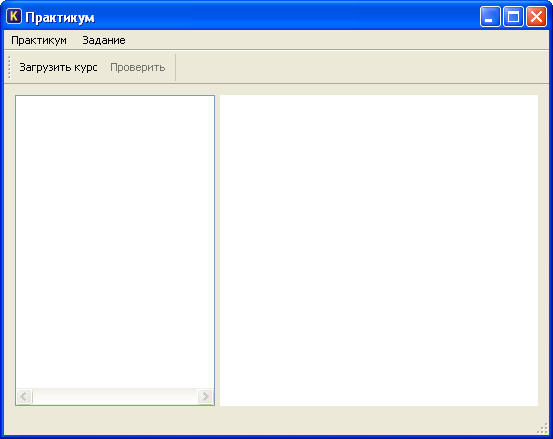
\includegraphics[scale=0.7]{pr1.png}
\caption{Окно практикумов. Исходное состояние}
\end{center}
\end{figure}

\begin{center}
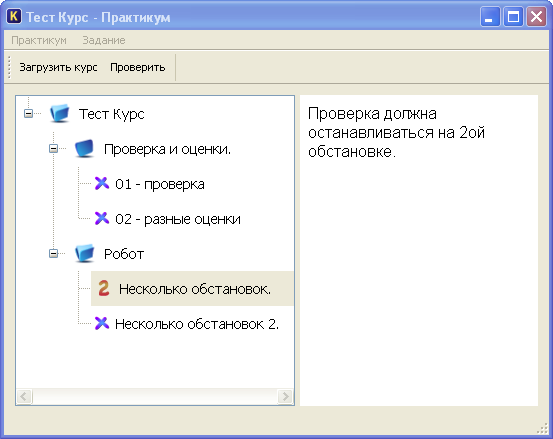
\includegraphics[scale=0.7]{pr3.png}


Рис 2.2 Окно практикумов. Тестовый курс
\end{center}

\subsection {Общее описание сеанса }
После того, как появилось окно «Практикум», пользователь выбирает практикум, далее он работает с выбранным практикумом – поочередно выбирает и выполняет задания. В каждый момент пользователю доступен для выполнения определенный набор заданий (см. выше). 
	
	В произвольный момент работы пользователь может сохранить состояние своей работы в виде личной копии практикума (рабочей тетради). Впоследствии эта копия может быть загружена и работа будет продолжена с того состояния, в котором она была прервана.


\subsection {Выполнение задания }
Пользователь выбирает задание, используя левое поле окна курса. После этого в правом поле этого окна появляется словесное описание задания, а в поле программы окна системы КуМир устанавливается обстановки исполнителей и начальный текст программы – сохраненный во время предыдущего сеанса текст или (при первом запуске задания) исходный шаблон. Если требуется , загружается обстановка нужного исполнителя. 
	Далее пользователь обычным образом создает нужную программу и, когда, по его мнению, программа готова, вызывает проверку (см. ниже). 
	
	По результатам проверки за задание выставляется оценка и, возможно, изменяется множество доступных заданий. Оценки показываются на дереве заданий рядом с соответствующими заданиями.
	
	Пользователь может продолжить выполнение задания (если проверка дала отрицательный результат) или выбрать новое задание. 


\subsection {Проверка задания} \label{test}
	Для проверки текущей программы необходимо нажать кнопку «Проверить» главного меню окна курсов, если до этого рабочая тетрадь не была создана то будет выдано предложение создать тетрадь. Задание может содержать несколько обстановок исполнителей. Если на очередной обстановке в работе программы обнаружена ошибка, то тестирование прерывается, в поле ввода-вывода выводится соответствующее сообщение и обстановка, на которой обнаружена ошибка предъявляется ученику. При каждом тестировании проверяется работоспособность программы на всех тестовых обстановках, независимо от результатов предыдущих тестирований.  Можно проверить задание только на текущей обстановке (без выставления оценки), нажав Ctrl+t.
	
	Проверка работы программы ученика (при данной обстановке исполнителя) состоит в вызове подготовленного учителем алгоритма-функции без параметров с именем 
	\emph{@тестирование}; этот алгоритм готовит разработчик курса (см. пп.\ref{seans} и \ref{setup}). Алгоритм \emph{@тестирование} возвращает целое число – оценку за работу программы при данной обстановке. Общая оценка – это минимум из оценок по всем обстановкам. 
	
	Как отмечалось выше, тестирующие алгоритмы заданий готовит автор курса. Поэтому критерии оценок полностью находятся в его руках.
	
	Система запоминает тестировавшуюся версию программы. При желании учитель может посмотреть эту версию, внести свои комментарии и т.п. О сохранении версий программ см. ниже. 


\subsection {Сохранение версий программы}
Ученик может в любой момент сохранить текущее состояние программы в файл, как это предусмотрено возможностями системы КуМир (или другой используемой управляющей системы). 
	
	В то же время в рабочей тетради для каждого задания запоминаются следующие версии программы:
	\begin{enumerate}
	\item исходная заготовка («шаблон»);
	\item версия программы,  с которой был начат сеанс (см. п. 1.5);
	\item последнюю тестировавшуюся версию программы.
\end{enumerate}
	Ученик может вернуться к каждой из указанных версий программы с помощью меню «Задание» окна практикумов. 
	
	Кроме того, в момент остановки работы над заданием (т.е. при выборе нового задания или проверки) запоминается текущее состояние программы. При повторном обращении к заданию работа будет продолжена с того же состояния, в котором она была прервана. 


\subsection {Сохранение состояния курса}
	В любой момент сеанса ученик может сохранить текущее состояние работы над практикумом. Состояние сохраняется в т.н. \emph{личном} файле ученика – рабочей тетради. 
	В этом файле хранится ссылка на описание практикума (самого практикума не хранится), оценки по заданиям и созданные учеником для каждого задания версии программ (последняя тестировавшаяся и «текущая», т.е. версия на момент прерывания работы над заданием). 
	
	При сохранении состояния ученике, как обычно, выбирает имя личного файла, в которое происходит сохранение. При загрузке курса из личного файла  сначала загружается основной практикум, а затем результаты предыдущей работы ученика. 



\section {Подготовка курса } \label {newk}
\subsection {Файл описания курса}
Файл описания курса  - это XML файл. В нем хранится  дерево заданий. Для создания таких файлов в поставке Кумир имеется утилита «Редактор практикумов». Для каждого задания описывается:
\begin{enumerate}
\item	Номер задания.
\item	Имя необходимой УС. Пока только Кумир.
\item	Имя задания
\item	Текстовое описание задания или ссылка на html файл.
\item	Ссылка на файл стартовой программы.
\item	Список имен необходимых исполнителей.
\item	Ссылки на файлы обстановок исполнителей.
\item	Текущая оценка.
\item	Минимальные и максимальные оценки по другим заданиям, необходимые для этого задания (указываются только задания, от которых зависит данное задание).

\end{enumerate}
\subsection {Файлы заданий}
Это файлы, на которые имеются ссылки в файле описания курса (файлы обстановок, HTML-файлы описаний, файлы программ и другие файлы необходимые для выполнения задания).  Для них может быть указан любой путь. Но на практике удобно, чтобы они лежали в том же каталоге, что и файл описания практикума или в подкаталоге этого каталога.

\subsection {Подготовка программы-заготовки} \label{setup}
Программу-заготовку рекомендуется готовить с помощью системы КуМир, запущенной в учительском режиме (ключ -t). В заготовку должны обязательно входить следующие фрагменты, защищенные от изменения учеником:
\begin{enumerate}
\item	заголовок требуемого алгоритма;
\item	 тестирующий алгоритм-функция без параметров \textbf{цел} \emph{@тестирование}. 
	\end{enumerate}
	Заголовок должен быть виден ученику, а алгоритм \emph{@тестирование}, как правило (но не обязательно!) скрыт от ученика. Сделать фрагменты программы защищенными от изменения и невидимыми можно в редакторе КуМира, используя правую кнопку мыши. Подробнее о подготовке алгоритма тестирования см. ниже.
	Кроме указанных необходимых элементов, в заготовку можно включать по желанию разработчика и другие элементы программы – описания величин, управляющие конструкции и т.п. Делать весь текст заготовки защищенным от изменений не обязательно.
	
	Пример заготовки программы – см. DemoKurs.zip 

\subsection {Подготовка тестирующего алгоритма }
           Тестирующий алгоритм – часть программы-заготовки. Это алгоритм-функция   языка КуМир типа 
           \textbf{цел}. Возвращаемое значение является оценкой, которую получит ученик. Тестирующий алгоритм должен иметь имя 
           \emph{@тестирование}. 
	Тестирующий алгоритм может вызывать другие алгоритмы. Имена этих алгоритмов должны начинаться с символа , чтобы не создавать конфликтов с именами алгоритмов пользователя. Эти имена не будут показываться ученику при вызове подсказки, которая выдает список доступных алгоритмов.
	
	
	Тестирующий алгоритм и вызываемые им алгоритмы разработчика должны быть расположены в конце программы-заготовки. Это связано с тем, что в системе КуМир скрыть от ученика можно лишь фрагмент текста от указанной позиции до конца программы.
	
	
	Поддержка практикумов обеспечивает многократный вызов тестирующего алгоритма, если задан список тестовых обстановок. Нужно иметь Это нужно иметь в виду при создании тестирующего алгоритма. Для проверки заданий, связанных с исполнителем Робот, существуют дополнительные команды см.  Список алго-ритмов Робота в системе Кумир . Эти команды нельзя использовать вне тестиру-ющего алгоритма.

\subsection {Подсказки}
Возможность что-то подсказать ученику – важный элемент методики, заложенной в практикум. 
\begin{enumerate}	
\item В заготовку программы можно включать не только заголовок, но и элементы решения.
\item Можно включать в практикум «задания», для которых программа-решение почти полностью включена в заготовку. 
Такая программа может быть доступна всегда. 
Другая возможность – задание-подсказка становится доступным только, 
если ученик попробовал выполнить «основное» задание. 
О наличии такого вспомогательного задания-подсказки можно сообщить в поясняющем тексте задания.
\end{enumerate}

